% CHAPTER ON ILC MACHINE

%{\it Status: Feb 12, 2019}  - revised by MEP

The International Linear Collider (ILC) is a $250\,{\mathrm{GeV}}$ (extendable up to $1\,{\mathrm{TeV}}$) linear $e^+e^-$ collider, based on $1.3\,{\mathrm{GHz}}$ superconducting radio-frequency (SCRF) cavities.
It is designed to  achieve a luminosity of $1.5\cdot 10^{34}~{\mathrm{cm}}^{-1}{\mathrm{s}}^{-1}$ and provide an integrated luminosity of $350\,{\mathrm{fb}}^{-1}$ in the first four years of running.
The electron beam will be polarised to $80\,\%$, and positrons with $30\,\%$ polarization will be provided if the undulator based positron source concept is employed. 

Its parameters have been set by physics requirements first outlined in 2003,
updated in 2006, and thoroughly discussed over many years with the physics user community. 
After the discovery of the Higgs boson it was decided that an initial energy of $250\,{\mathrm{GeV}}$ provides the opportunity for a precision physics programme at a reasonable initial cost~\cite{Evans:2017rvt}.
Some relevant parameters are given in Tab.~\ref{tab:ilc-params}.

\begin{table*}[tbhp]
\begin{tabular}{lcccccc}
Quantity & Symbol & Unit & Initial & TDR &  \multicolumn{2}{c}{Upgrades} \\
\hline
Centre of mass energy & $\sqrt{s}$ & ${\mathrm{GeV}}$ & $250$ & $250$ & $500$ & $1000$ \\
Luminosity & \multicolumn{2}{c}{${\mathcal{L}}$ ~~~~$10^{34}{\mathrm{cm^{-2}s^{-1}}}$} & $1.35$ & $0.75$ & $1.8$ & $4.9$ \\
Polarisation for $e^- (e^+)$ & $P\sub{-} (P\sub{+})$ & & ~$80\,\% (30\,\%)$~ &  ~$80\,\% (30\,\%)$~ &  ~$80\,\% (30\,\%)$~ &  ~$80\,\% (20\,\%)$~  \\
Repetition frequency &$f\sub{{rep}}$ & ${\mathrm{Hz}}$  & $5$ & $5$ & $5$ & $4$ \\
Bunches per pulse  &$n\sub{{bunch}}$ & 1  & $1312$ & $1312$ & $1312$ & $2450$ \\
Bunch population  &$N\sub{{e}}$ & $10^{10}$ &$2$ & $2$ & $2$ & $1.74$ \\
Linac bunch interval & $\Delta t\sub{{b}}$ & ${\mathrm{ns}}$ & $554$ & $554$ & $554$ & $366$ \\
Beam current in pulse & $I\sub{{pulse}}$ & ${\mathrm{mA}}$& $5.8$ & $5.8$ & $5.8$ & $7.6$  \\
Beam pulse duration  & $t\sub{{pulse}}$ & ${\mathrm{\mu s}}$ & $727$ & $727$ & $727$ & $897$ \\
Average beam power  & $P\sub{{ave}}$   & ${\mathrm{MW}}$ & $5.3$ & $5.3$ & $10.5$  & $27.2$ \\  
Norm. hor. emitt. at IP & $\gamma\epsilon\sub{{x}}$ & ${\mathrm{\mu m}}$& $5$ & $10$ & $10$ & $10$  \\ 
Norm. vert. emitt. at IP & $\gamma\epsilon\sub{{y}}$ & ${\mathrm{nm}}$ & $35$ & $35$ & $35$ & $35$ \\ 
RMS hor. beam size at IP  & $\sigma^*\sub{{x}}$ & ${\mathrm{nm}}$  & $516$ & $729$ & $474$ & $335$ \\
RMS vert. beam size at IP &$\sigma^*\sub{{y}}$ & ${\mathrm{nm}}$ & $7.7$  & $7.7$  & $5.9$ & $2.7$ \\
Luminosity in top $1\,\%$ & ${\mathcal{L}}\sub{0.01} / {\mathcal{L}}$ &  & $73\,\%$  & $87.1\,\%$  & $58.3\,\%$ & $44.5\,\%$\\
Energy loss from beamstrahlung  & $\delta\sub{BS}$ &  & $2.6\,\%$  & $0.97\,\%$  & $4.5\,\%$ & $10.5\,\%$ \\
Site AC power  & $P\sub{{site}}$ &  ${\mathrm{MW}}$ & $129$ & $122$ & $163$ & $300$ \\
Site length & $L\sub{{site}}$ &  ${\mathrm{km}}$ & $20.5$ & $31$ & $31$ & $40$ \\
\end{tabular}
\caption{Summary table of the ILC accelerator parameters in the initial $250\,{\mathrm{GeV}}$ staged configuration (with TDR parameters at \siunit{250}{GeV} given for comparison) and possible upgrades.
\label{tab:ilc-params}}
\end{table*}

The collider design is the result of nearly twenty years of R\&D. 
The heart of the ILC, the system of superconducting cavities, is based on over a decade of pioneering work by the TESLA collaboration in the 1990s. 
Some other aspects were based on the R\&D carried out for the JLC/GLC and NLC projects, which were based on room-temperature accelerating structures. 
From 2005 to the publication of the Technical Design Report (TDR)~\cite{Adolphsen:2013kya} in 2013, the design of the ILC accelerator was conducted as a worldwide international collaboration coordinated by the Global Design Effort (GDE) under a mandate from the International Committee for Future Accelerators (ICFA).
Since then, the Linear Collider Collaboration (LCC) has been coordinating the international activities for both, the ILC and CLIC projects, again mandated by ICFA.

The fundamental goal of the design of the ILC accelerator is a high energy efficiency.  The ILC design
 limits the overall power consumption of the accelerator complex during operation to $129\,{\mathrm{MW}}$ at  $250\,{\mathrm{GeV}}$ and $300\,{\mathrm{MV}}$ at  $1\,{\mathrm{TeV}}$, which is comparable to the power consumption of CERN.
% Stapnes at ALCW2018: 1.35TWh in 2012 -> 154MW on average in 2012
This is achieved by the use of SCRF technology for the main accelerator, which offers a high RF-to-beam efficiency through the use of superconducting cavities, operating at $1.3\,{\mathrm{GHz}}$, where high-efficiency klystrons are commercially available.
At accelerating gradients of $31.5$ to $35\,{\mathrm{MV/m}}$ this technology offers high overall efficiency and reasonable investment costs, even considering the cryogenic infrastructure needed for the operation at $2\,{\mathrm{K}}$.

The underlying TESLA technology is mature, with a broad industrial base throughout the world, and is in use at a number of free electron laser facilities that are in operation (European XFEL at DESY, Hamburg), under construction (LCLS-II at SLAC, Stanford) or in preparation (SCLF in Shanghai) in the three regions Asia, Americas, and Europe that contribute to the ILC project.
In preparation for the ILC, Japan and the U.S. have founded a collaboration for further cost optimisation of the TESLA technology.
In recent years, new surface treatment technologies utilising nitrogen during the cavity preparation process, such as the so-called   nitrogen infusion technique, have been developed at Fermilab, with the prospect of  achieving higher gradients and lower loss rates with a less expensive surface preparation scheme than assumed in the TDR (see Par.~\ref{par:infusion}).

When the Higgs boson discovery was imminent in 2012, the Japan Association of High Energy Physicists (JAHEP) made a proposal to host the ILC in Japan~\cite{JAHEP:2012a,JAHEP:2012b}. 
Subsequently, the Japanese ILC Strategy Council conducted a survey of possible sites for the ILC in Japan, looking for  suitable geological conditions for a tunnel up to $50\,{\mathrm{km}}$ in length (as required for a $1\,{\mathrm{TeV}}$  machine), and the possibility to establish a laboratory where several thousand international scientists can work and live. 
As a result, the candidate site in the Kitakami region in northern Japan, close to the larger cities of Sendai and Morioka, was found to be the best option. 
The site offers a large, uniform granite formation with no currently active faults and a geology that is well suited for tunnelling.
Even in the great Tohoku earthquake in 2011, underground installations in this rock formation were essentially unaffected~\cite{bib:sanuki:desy2017}, which underlines the suitability of this candidate site. 

This section starts with a short overview over the changes of the ILC design between the publication of the TDR in $2013$ and today, followed by a description of the SCRF technology, and an description of the overall accelerator design and its subsystems. 
Thereafter, possible upgrade options are laid out, the Japanese candidate site in the Kitakami region is presented, and costs and schedule of the accelerator construction project are shown.


%===============================================================================
 \begin{figure*}[tbhp]
 %\epsfysize=9.0cm
 \begin{center}
 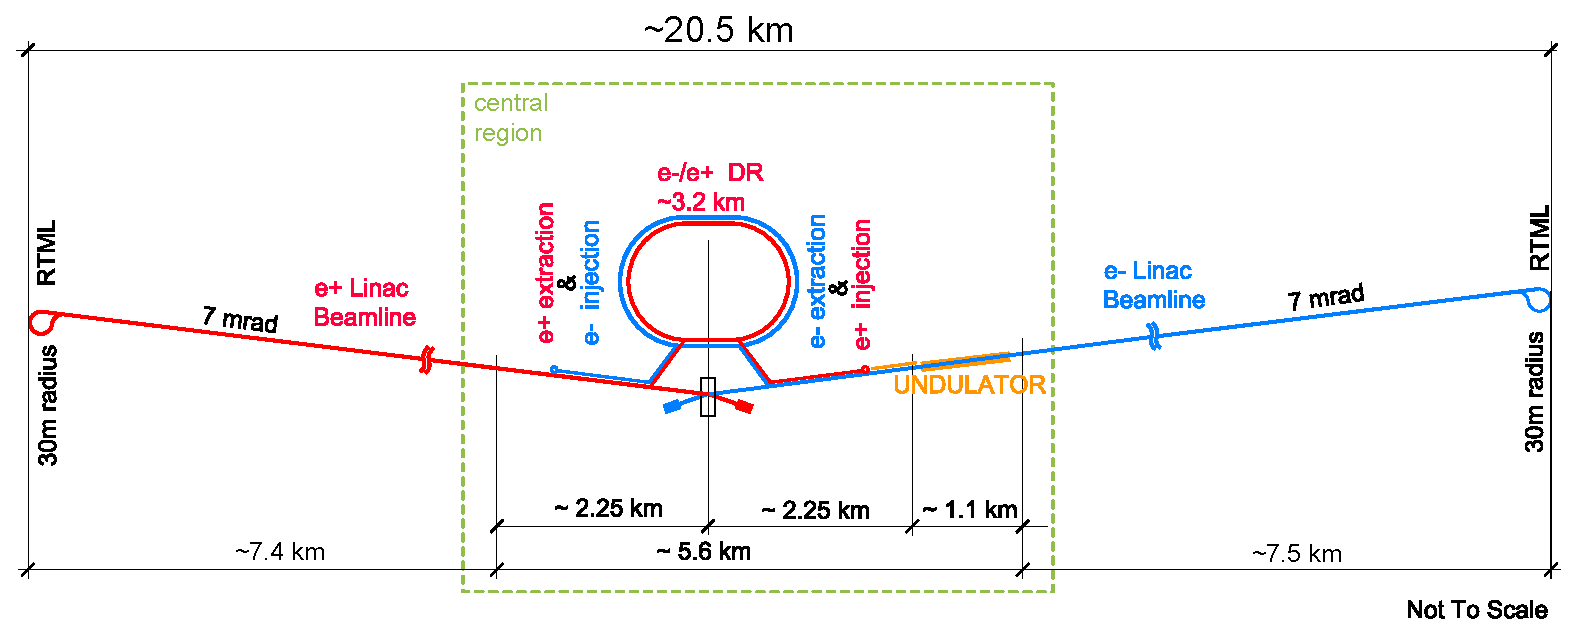
\includegraphics[width=\hsize]{chapters/figures/TDR-machine-layout-cartoon-staged-mirror.pdf}
\caption{Schematic layout of the ILC in the $250\,{\mathrm{GeV}}$ staged configuration.
\label{fig:ilc-schematic}}
 \end{center}
 \end{figure*}

\subsection{Design Evolution since the TDR}
\label{sec:design_evo}

Soon  after the discovery of the Higgs boson, the Technical Design Report (TDR) for the ILC accelerator was published in 2013~\cite{Adolphsen:2013jya,Adolphsen:2013kya} after 8 years of work by the Global Design Effort (GDE).
The TDR design was based on the requirements set forth by the ICFA mandated parameters committee~\cite{Heuer:2006}:
\begin{itemize}
\item a centre-of-mass energy of up to \siunit{500}{GeV},
\item tunability of the centre-of-mass energy between $\sqrt{s} = \siunit{200}{GeV}$
 and \siunit{500}{GeV},
\item  a luminosity sufficient to collect \siunit{500}{fb^{-1}} within four years of operation, taking into account a three-year a ramp up.  This corresponds to a final luminosity of \siunit{250}{fb^{-1}} per year and an instantaneous luminosity of ${\mathcal{L}} = \siunit{2 \cdot 10^{34}}{cm^{-2}\,s^{-1}}$,
\item an electron polarisation of at least $80\,\%$,
\item  the option for a later upgrade to energies  up to \siunit{1}{TeV}.
\end{itemize}

The accelerator design presented in the TDR met these requirements (see Tab.~\ref{tab:ilc-params}), at an estimated construction cost of \siunit{7,982}{MILCU} for a Japanese site, plus \siunit{22.9}{Mh} (million hours) of labour in participating institutes~\cite[Sec. 15.8.4]{Adolphsen:2013kya}. 
Costs were expressed in ILC Currency Units ILCU, where \siunit{1}{ILCU} corresponds to \siunit{1}{US\$} at 2012 prices.

In the wake of the Higgs discovery, and the proposal by the Japan Association of High Energy Physicists (JAHEP) to host the ILC in Japan\cite{JAHEP:2012a} with its recommendation to start with a \siunit{250}{GeV} machine~\cite{JAHEP:2012b}, plans were made for a less expensive machine configuration with a centre--of--mass energy of $\sqrt{s} = \siunit{250}{GeV}$, around the maximum of the $Zh$ production cross section, half the TDR value.
Various options were studied in the TDR~\cite[Sect. 12.5]{Adolphsen:2013kya} and later~\cite{Dugan:2014}.
This resulted in a revised proposal~\cite{Evans:2017rvt} for an accelerator with an energy of \siunit{250}{GeV} and a luminosity of ${\mathcal{L}} = \siunit{1.35 \cdot 10^{34}}{cm^{-2}\,s^{-1}}$, capable of delivering about \siunit{400}{fb^{-1}} per year, or \siunit{200}{fb^{-1}} within the first four years of operation, taking into account the ramp-up.

Several other changes of the accelerator design have been approved by the ILC Change Management Board since 2013, in particular:
\begin{itemize}
\item The free space between the interaction point and the edge of the final focus quadrupoles ($L^*$) was unified between the ILD and SiD detectors~\cite{bib:cr-0002}, facilitating a machine layout with an optimised luminosity for both detectors. 
\item A vertical access shaft to the experimental cavern was foreseen~\cite{bib:cr-0003}, allowing a CMS-style assembly concept for the detectors, where large detector parts are built in an above-ground hall while the underground cavern is still being prepared. 
\item The shield wall thickness in the Main Linac tunnel was reduced from $3.5$ to \siunit{1.5}{m}~\cite{bib:cr-0012}, leading to a significant cost reduction. This was made possible by dropping the requirement for personnel access during beam operation of the main linac.
\item Power ratings for the main beam dumps, and intermediate beam dumps for beam aborts and machine tuning, were reduced to save costs~\cite{bib:cr-0013}.
\item A revision of the expected horizontal beam emittance at the interaction point at \siunit{125}{GeV} beam energy, based on improved performance expectations for the damping rings and a more thorough scrutiny of beam transport effects at lower beam energies, lead to an increase of the luminosity expectation from $0.82$ to \siunit{1.35 \cdot 10^{34}}{cm^{-2}\,s^{-1}}~\cite{bib:cr-0016}.
\end{itemize}

All these changes contributed to an overall cost reduction, risk reduction, and improved performance expectation.

Several possibilities were evaluated for the length of the initial tunnel. 
Options that include building tunnels with the length required for a machine with $\sqrt{s} = \siunit{350}{GeV}$ or \siunit{500}{GeV}, were considered.
In these scenarios, an energy upgrade would require the installation of additional cryomodules (with RF and cryogenic supplies), but little or no civil engineering activities.
In order to be as cost effective as possible, the final proposal, endorsed by ICFA~\cite{ICFA:2017}, does not include these empty tunnel options. 

While the length of the main linac tunnel was reduced, the beam delivery system and the main dumps are still designed to allow for an energy upgrade up to  $\sqrt{s} = \siunit{1}{TeV}$.


\subsection{Superconducting RF Technology}


%{\it Description of the TESLA SCRF technology - 4 pages
%
%Stresses long experience - FLASH, STF, XFEL, broad industrial base - LCLS-II, SHINE:
%addresses concerns mentioned in Nomura report and others (yield / gradient, MARX modulator)
%
%Nomura issue: MARX modulator
%
%Figures: Cavity, Cryomodule (Rey Hory) 
%
%}


The heart of the ILC accelerator consists of the two superconducting Main Linacs that accelerate both beams from \num{5} to \siunit{125}{GeV}.
These linacs are based on the TELAS technology:
beams are accelerated in \siunit{1.3}{GHz} nine-cell superconducting cavities made of niobium and operated at \siunit{2}{K} (Fig.~\ref{fig:tesla-cavity}). These 
 are assembled into cryo modules comprising eight to nine cavities, an optional quadrupole / corrector / beam position monitor unit, and all necessary cryogenic supply lines (Fig.~\ref{fig:crymodule}). 
Pulsed klystrons supply the necessary radio frequency power (High-Level RF HLRF) to the cavities by means of a waveguid power distribution system and input couplers, one per cavity.

This technology was primarily developed at DESY for the TESLA accelerator project that was proposed in 2001.
Since then, the TESLA technology collaboration~\cite{bib:ttc} has been improving this technology, which is now being used in several accelerators in operation (FLASH at DESY~\cite{schreiber_faatz_2015,Vogt:2018wvy}, European XFEL in Hamburg~\cite{bib:xfel}), under construction (LCLS-II at SLAC, Stanford, CA~\cite{bib:lcls-ii}) or planned (SHINE in Shanghai~\cite{Zhao:2018lcl}).


%\subsubsection{The Economics of Superconducting Linacs}
%
%The total energy dissipation $P\sub{d}$ in a linac cavity of length $L$ and a total voltage $V = g L$ at a the accelerating gradient $g$ is given by
%$$
%  P\sub{d} = g V R\sub{s} \lambda / C
%$$
%where $R\sub{s}$ is the material's surface resistance, $\lambda$ is the RF frequency, and $C$ (in ${\mathrm{\Omega^2}}$) depends only on the cavity shape, not its size.
%The dissipated power in a single cavity grows with the square of the gradient, 
%and the overall power grows linearly with the gradient for a given accelerating voltage.

\begin{figure*}[tbhp]
   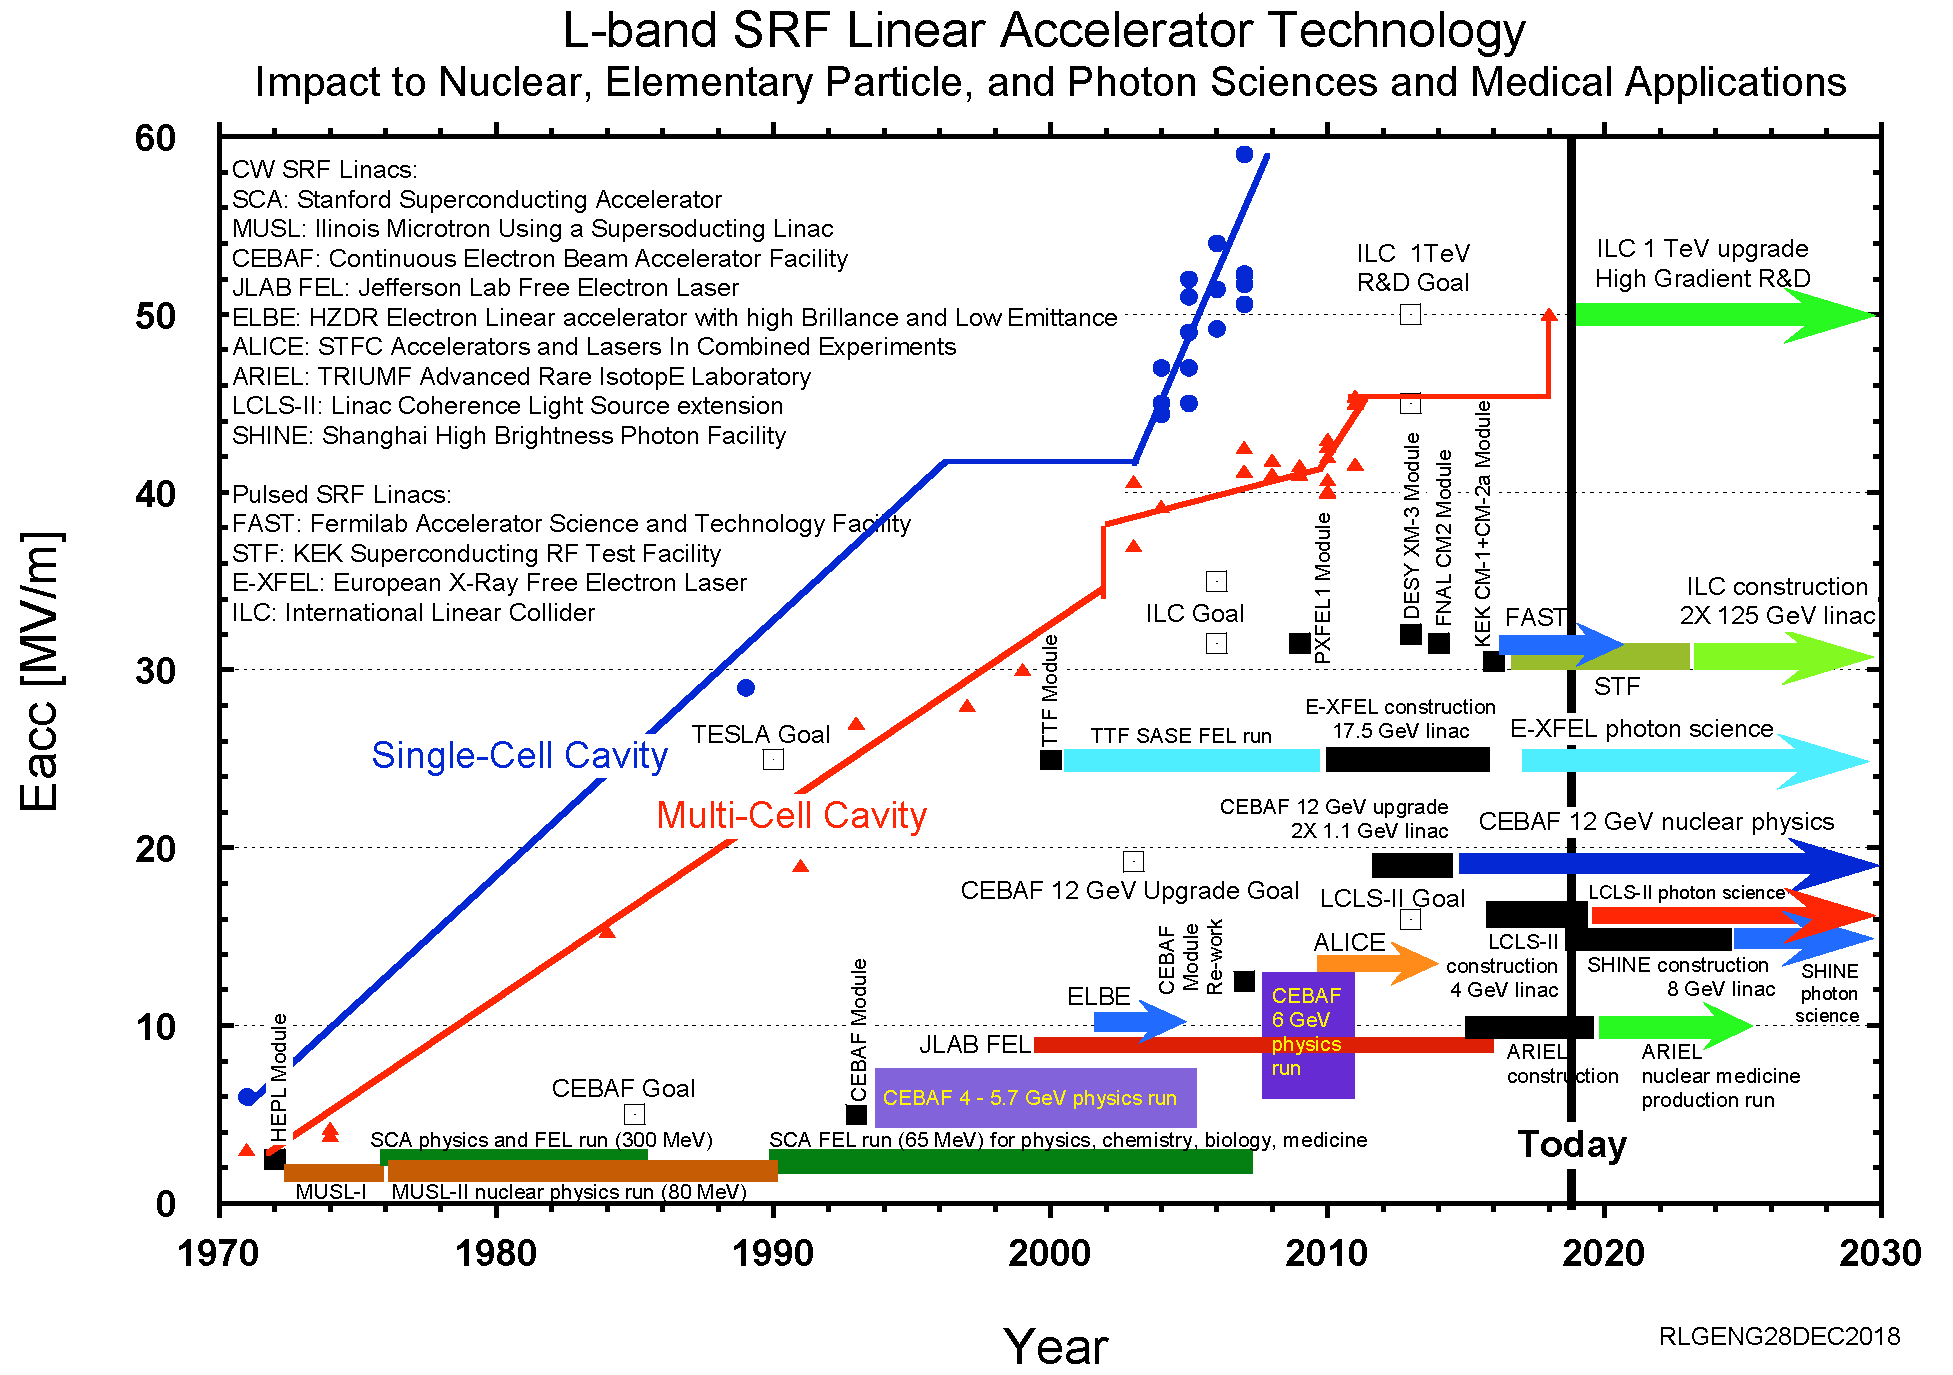
\includegraphics[width=0.8 \hsize]{chapters/figures/LBandSRFNbCavityGradientEvolution_ProjectImpact_rev28dec2018}
\caption{Development of the gradient of SRF cavities since 1970
\cite[updated]{Geng:2015glc}.
}
% Paper is published under CC-BY-3.0
\label{fig:gradients}
\end{figure*}

\subsubsection{The Quest for High Gradients}

The single most important parameter for the cost and performance of the ILC is the accelerating gradient $g$.
The TDR baseline value is an average gradient $g = \siunit{31.5}{MV/m}$ for beam operation, with a $\pm 20\,\%$ gradient spread between individual cavities.
Recent progress in R\&D for high gradient cavities raises the hope to raise the gradient by  $10\,\%$  to  $g = \siunit{35}{MV/m}$, which would reduce the total cost of the \siunit{250}{GeV} accelerator by about  $6\,\%$.
%% 6% = 50BY / 803BY
% Copied from TDR Vol 3.II p. 23
To achieve the desired gradient in beam operation, the gradient achieved in the low-power vertical test (mass production acceptance test) is specified $10\,\%$ higher to allow for operational gradient overhead for low-level
RF (LLRF) controls, as well as some degradation during cryomodule installation (few ${\mathrm{MV/m}}$).
Fig.~\ref{fig:gradients} shows how the achievable gradients have evolved over the past 50 years~\cite{Geng:2015glc}.

\paragraph{Gradient impact on costs:}
To the extent that the cost of cavities, cryomodules and tunnel infrastructure is independent of the achievable gradient, the investment cost per GeV of beam energy is inversely proportional to the average gradient achieved. This is the reason for the enormous cost saving potential from higher gradients.
This effect is partially offset by two factors:  the energy stored in the electromagnetic field of the cavity, and the dynamic heat load to the cavity from the electromagnetic field.  These grow quadratically with the gradient, and thus linearly for a given beam energy.
The electromagnetic energy stored in the cavity must be replenished by the RF source during the filling time that precedes the time when the RF is used to accelerate the beam passing through the cavity; this energy is lost after each pulse and thus reduces the overall efficiency and requires more or more powerful modulators and klystrons.
The overall cryogenic load is dominated by the dynamic heat load from the cavities, and thus operation at higher gradient requires larger cryogenic capacity.
Cost models that parametrise these effects indicate that the minimum of the investment cost per GeV beam energy lies at \num{50} or more GeV, depending on the relative costs of tunnel, SCRF infrastructure and cryo plants, and depending on the achievable $Q_0$~\cite{Adolphsen:2011a}. 
Thus,  the optimal gradient is significantly higher than the value of approximately \siunit{35}{MV/m} that is currently realistic; this emphasises  the relevance of achieving higher gradients.

It should be noted that in contrast to the initial investment, 
the operating costs rise when the gradient is increased, and this must be factored into 
the cost model.

\paragraph{Gradient limitations:}
Fundamentally, the achievable gradient of a SC cavity is limited by the point where the magnetic field at the cavity walls surpasses the critical field $H\sub{crit,RF}$ of the superconductor.
This gradient depends on the material, operating temperature, and the cavity geometry. 
For the TESLA type cavities employed at the ILC, this limit is about \siunit{48}{MV/m} at \siunit{2}{K}.
The best XFEL production cavity reached \siunit{44.6}{MV/m} (Fig.~\ref{fig:cavity-gradient}).
The record for single cell cavities operating at \siunit{1.3}{GHz} is \siunit{59}{MV/m}~\cite{Eremeev:2007zza}.
%
% Explanation:  
% 48MV/m using  $B\sub{pk}/g = \SIunit{4.26}{mT / (MV/m)}$ for ILC cavities~\cite{Adolphsen:2013kya}
% and the critical field for niobium at \SIunit{2}{K} has been measured to be \SIunit{205}{mT}~\cite{Padamsee:2009,Hays:1995zd}.
% , not far from the theoretical prediction of \SIunit{230}{mT}~\cite{Geng:2006wf}
% Padamsee:1998vf page 101 quotes 47MV/m for 4.2mT/MV/m
% Record 59MV/m corresponds to 206.5mT

Niobium is a type-II superconductor, and so it has two distinct superconducting phases, the Meissner state, with complete magnetic flux expulsion, which exists up to a field strength $H\sub{c1} \approx \siunit{180}{mT}/\mu_0$ ($\mu_0 = 4\pi \siunit{10^{-7}}{T\,m/A}$ being the vacuum permeability), and a mixed state in which flux vortices penetrate the material, up to a higher field strength $H\sub{c1}$, at which superconductivity breaks down completely.
In time-dependent fields, the penetrating vortices move due to the changing fields and thus dissipate energy, causing a thermal breakdown. 
However, for RF fields, the Meissner state may persist metastably up to the superheating field strength $H\sub{sh} \approx \siunit{240}{mT}/\mu_0$, which is expected to be the critical RF field critical field $H\sub{crit,RF}$~\cite{Padamsee:1998vf}.
Experimentally, niobium RF cavities have been operated at field strengths as high as $H=\siunit{206}{mT}/\mu_0$~\cite{Eremeev:2007zza}, and the best XFEL production cavities reach about $\siunit{190}{mT}$.
Recently, even \siunit{210}{mT} has been achieved at FNAL~\cite{Grassellino:2018tqg}.
In recent years, theoretical understanding of the nature of this metastable state and the mechanisms at the surface that prevent flux penetation has significantly improved~\cite{Gurevich:2017vnn,Kubo:2017cww}.
It appears that a thin layer of ``dirty'' niobium, \ie,  with interstitial impurities, on top of a clean bulk with good thermal conductivity, is favourable for high field operation.  

The gradient at which a SC cavity can be operated in practice is limited by three factors   in addition to those just listed~\cite{Padamsee:1998vf}:
\begin{itemize}
\item the thermal breakdown of superconductivity, when local power dissipation causes a local quench of the superconductor,
\item the decrease of the quality factor $Q_0$ at high gradients that leads to increased power dissipation,
\item the onset of field emission that causes the breakdown of the field in the cavity.
\end{itemize}
The onset of these adverse effects is mostly caused by micro-metre sized surface defects of various kinds. 
Producing a sufficiently defect-free surface in an economic way is thus the central challenge in cavity production.

More than 20 years of industrial production of TESLA type cavities have resulted in a good understanding which production steps  and quality controls are necessary to produce cavities with high-quality, nearly defect-free surfaces that are capable of achieving the desired high field strengths at a reasonable production yield.


\paragraph{Results from XFEL cavity production:}

\begin{figure}[htbp]
   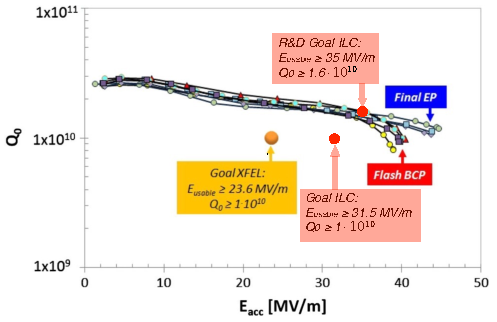
\includegraphics[width=\hsize]{chapters/figures/prab-19-092001-fig19-mod}
\caption{Examples of the $Q_0\,(E\sub{acc})$ curves of some of the best
cavities, either treated at RI using ``EP final'', or at EZ using
``BCP flash.''
\cite[Fig. 19]{Singer:2016fbf}. 
Vendor ``RI'' employs a production process that closely follows the ILC specifications, with a final electropolishing step.
The ILC gradient / $Q_0$ goals are overlaid.}
% Paper published under CC-BY-3.0
\label{fig:cavity-gradient}
\end{figure}

The production and testing of $831$ cavities for the European XFEL~\cite{Singer:2016fbf,Reschke:2017gjp} provides the biggest sample of cavity production data so far. 
Cavities were acquired from two different vendors RI and EZ,
of which vendor RI employed a production process with a final surface treatment closely following the ILC specifications, including a final electropolishing (EP) step,
while the second vendor EZ used buffered chemical polishing (BCP).
The XFEL specifications asked for a usable gradient of \siunit{23.6}{MV/m} with a $Q_0 \ge 1  \cdot 10^{10}$ for operation in the cryomodule;
with a $10\,\%$ margin this corresponds to a target value of \siunit{26}{MV/m} for the performance in the vertical test stand for single cavities.
Fig.~\ref{fig:cavity-gradient} shows the $Q_0$ data versus accelerating gradient of the best cavities received, with several cavities reaching more than \siunit{40}{MV/m}, significantly beyond the ILC goal, already with $Q_0$ values that approach the target value $1.6\cdot10^{10}$ that is the goal of future high-gradient R\&D.

\begin{figure}[htbp]
   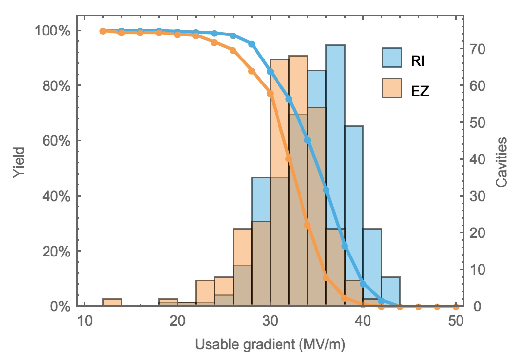
\includegraphics[width=\hsize]{chapters/figures/prab-20-042004-fig33}
\caption{Distribution and yield of the ``as received'' maximum
gradient of cavities produced for the European XFEL, separated by vendor \cite[Fig. 33]{Reschke:2017gjp}. 
Vendor ``RI'' employs a production process that closely follows the ILC specifications, with a final electro polishing step.}
% Paper published under CC-BY-4.0
\label{fig:cavity-yield}
\end{figure}


XFEL production data, in particular from vendor RI, provide excellent statistics for the cavity performance as received from the vendors, as shown in Fig.~\ref{fig:cavity-yield}.
For vendor ``RI'', the yield for cavities above \siunit{28}{MV/m} is $85\,\%$ of for the maximum gradient, with an average of \siunit{35.2}{MV/m}.

Since the XFEL performance goal was substantially lower than the ILC specifications, cavities with gradient below \siunit{28}{MV/m}, which would not meet ILC specifications, were not generally re-treated for higher gradients, limiting our knowledge of the effectiveness of re-treatment for large gradients.
Still, with some extrapolation it is possible to extract yield numbers applicable to the ILC specifications ~\cite{bib:Walker:2017.lcws}.

The XFEL data indicate that after re-treating cavities with gradients outside the ILC specification of $\siunit{35}{MV/m} \pm 20\,\%$, \ie, below \siunit{28}{MV/m}, a yield of $94\,\%$ for a maximum gradient above \siunit{28}{MV/m} can be achieved, with an average value of \siunit{35}{MV/m}, meeting the ILC specification.
Taking into account limitations from $Q_0$ and the onset of field emission, the usable gradient is lower.  Taking account of this gives a $82\,(91)\,\%$ yield and an average usable gradient of \siunit{33.4}{MV/m} after up to one (two) re-treatments.
The re-treatment and testing rate is significantly higher than assumed in the TDR, but the XFEL experience shows that re-treatment can mostly be limited to a simple high-pressure rinse (HPR) rather than an expensive electropolishing step.  

Overall, the XFEL cavity production data prove that it is possible to mass-produce cavities meeting the ILC specifications as laid out in the TDR with the required performance and yield.


\paragraph{High-gradient R\&D -- nitrogen infusion:}
\label{par:infusion}

\begin{figure}[htbp]
   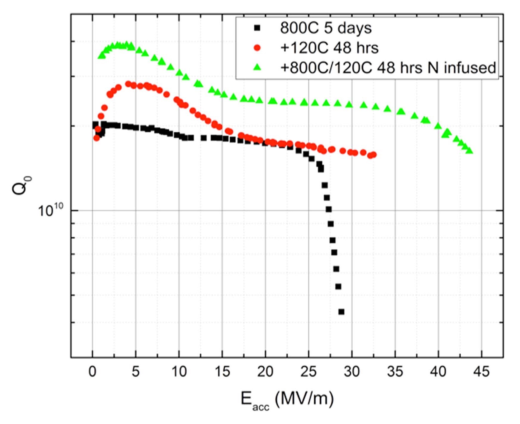
\includegraphics[width=\hsize]{chapters/figures/sst-30-094004-fig5}
\caption{Effect of successive cavity treatments on a single cavity: $\siunit{800}{^\circ C}$ bake for five days (black, lowest curve), followed by $48$ hours baking at $\siunit{120}{^\circ C}$ (red, middle curve). 
A third heat treatment including nitrogen infusion (green, top curve) significantly  raises the breakdown gradient and the quality factor of the cavity
\cite[Fig. 5]{Grassellino:2017bod}.
}
% Paper is published under CC-BY-3.0
\label{fig:n2infusion}
\end{figure}

In recent years, new techniques have emerged that seem to indicate that higher fields combined with higher quality factors are attainable in bulk niobium cavities.

In the early 2010s, nitrogen doping was developed as a method to substantially increase $Q_0$ by adding nitrogen during the \siunit{800}{^\circ C} baking, which leads to interstitial nitrogen close to the niobium surface~\cite{Grassellino:2013nza}.
This technique has been employed successfully in the production of the cavities for LCLS-II, with an average $Q_0$ of $3.0\cdot 10^{10}$ achieved in a prototype cryomodule~\cite{Wu:2018qyl}.
However, nitrogen doping reduces the critical RF field of the material and thus limits the achievable gradients to values below \siunit{30}{MV/m}, rendering doped material useless for high gradient applications.

By contrast, in nitrogen infusion the nitrogen is added during the low temperature baking at \siunit{120}{^\circ C}.
Experimental results seem to indicate that nitrogen infusion may offer a combination of three advantages:
\begin{itemize}
\item Reaching higher accelerating gradients,
\item higher $Q_0$ values, resulting in a reduced cryogenic load, 
\item a simplified and less expensive production process that does away with the final electropolishing step.
\end{itemize}

Fig.~\ref{fig:n2infusion} \cite[Fig. 5]{Grassellino:2017bod} shows how the addition of nitrogen during the final \siunit{48}{h} long \siunit{120}{^\circ C} bake of a one--cell cavity drastically improves the cavity quality factor as well as the maximum gradient, which comes close to the best XFEL cavity results, but at higher $Q_0$.

% XXX CONTINUE HERE XXX experimental status, success, transfer to other labs

Up to now, it has proven difficult to reproduce these exciting results in other laboratories.
Success has been reported by groups at JLAB~\cite{Dhakal:2017xxq}, and  Cornell~\cite{Koufalis:2017blg}, but KEK has reported mixed results \cite{bib:Umemori:2018.lcws}, and DESY has so far not been able to reproduce these results~\cite{Wenskat:2018zco}.
These difficulties seem to indicate that the recipe for a successful application of nitrogen infusion is not yet fully understood, and that further research and development will be necessary before this process can be transferred to industry. 

Nevertheless, the infusion results have triggered a renewed interest in the research on highest gradients in niobium cavities, with a host of new experimental results, increased activity to achieve a more thorough theoretical understanding~\cite{Kubo:2017cww,Gurevich:2017vnn}, and application of state-of-the-art analytical methods such as   muon spin rotation (muSR) \cite{Romanenko:2013saa}.
This provides reason for optimism that an improved understanding of the mechanisms that stabilise superconductivity in the presence of high fields will result in improved performance of industrially produced cavities for the ILC.

\paragraph{High-gradient R\&D -- alternative cavity shapes:}

Fundamentally, the achievable gradient in a niobium cavity is limited by the maximum magnetic field at the cavity surface, not the electrical field strengths.
The ratio between peak surface field $B\sub{pk}$ and gradient $g$ depends on the cavity geometry and is $B\sub{pk}/g = \siunit{4.26}{mT / (MV/m)}$ for TESLA type cavities.
A number of alternative cavity shapes have been investigated with lower ratios~\cite{Geng:2006wf},
resulting in single cells gradients up to \siunit{59}{MV/m}~\cite{Eremeev:2007zza}.
The reduced magnetic field, however, has to be balanced with other factors that favour the TESLA cavity shape, namely: a reasonable peak electrical field to limit the risk of field emission, sufficient iris width and cell-to--cell RF coupling, and a mechanical shape that can be efficiently fabricated.

Recently, new five-cell cavities with a new ``low surface field'' (LSF) shape~\cite{Li:2008a} have been produced at JLAB and have achieved gradient of up to~\siunit{50}{MV/m} in three of the five cells, which is a new record for multi-cell cavities~\cite{bib:Geng:2018.lcws}. 
The LSF shape aims to achieve a good compromise between the goal of a low magnetic field and the other criteria, and demonstrates that further improvements in gradient may be realised  in the future.


\subsubsection{Further Cost Reduction R\&D}

Additional strategies for cost reduction and improved cavity performance are also being investigated.

\paragraph{Low $RRR$ material:}

The niobium raw material and preparation of sheets  are a significant cost driver; R\&D is underway to re-evaluate the stringent limits on impurities, especially of tantalum, and the demand for a high residual resistivity ratio $RRR > 300$~\footnote{$RRR$ is the ratio of the material's room temperature resistivity to the normal conducting resistivity close to \siunit{0}{K}; heat conductivity from electrons is proportial to $RRR$. $RRR$ is reduced by impurities, in particular interstitial ones  from hydrogen, nitrogen and oxygen.}, to reduce the raw material cost.  The electrical 
conductivity and heat transport by electrons are proportional.  This implies that 
large $RRR$ values, indicative of low impurity content, make the cavities also 
less susceptible to thermal breakdown from surface defects.
However, when defect sizes can be successfully controlled to the extent necessary to achieve gradients above \siunit{35}{MV/m} routinely, the influence of heat conductivity and $RRR$ may be diminished, permitting the use of lower $RRR$ material~\cite{bib:Kubo:2018.ttc}.

\paragraph{Ingot and large-grain niobium:}

Together with direct slicing of discs from large niobium ingots, without rolling, forging and grinding or polishing steps, the cost for niobium sheets has the potential to be reduced by $50\,\%$~\cite{Evans:2017rvt,Kneisel:2014uqa}.
Without the mechanical deformation during rolling and forging, the grains from the initial crystallisation stay large, which makes later production steps, in particular deep--drawing of half cells, more challenging.
Nevertheless, if these challenges are overcome, tests with large--grain and ingot niobium show promising results~\cite{Reschke:2011a, Dhakal:2015xac}.


\subsubsection{Basic Parameters}

% Copied from TDR Vol 3.II p. 23
The choice of operating frequency is a balance between the higher cost of larger, lower-frequency cavities and the increased cost at higher frequency associated with the lower sustainable gradient from the increased surface resistivity. 
The optimum frequency is in the region of \siunit{1.5}{GHz}, but during the early R\&D on the technology, \siunit{1.3}{GHz} was chosen due to the commercial availability of high-power klystrons at that frequency.

\subsubsection{Cavities}

The superconducting accelerating cavities for the ILC are nine-cell structures made out of high-purity niobium (Fig.~\ref{fig:tesla-cavity}), with an overall length of \siunit{1.25}{m}.
Cavity production starts from niobium ingots which are forged and rolled into \siunit{2.8}{mm} thick niobium sheets that are individually checked for defects by an eddy current scan and optical inspection~\cite{Adolphsen:2013jya}.
Cavity cells are produced by deep-drawing the sheets into half cells, \num{18} of which are joined by electron beam welding with two end groups to form the whole structure.
This welding process is one of the most critical and cost-intensive steps of the cavity manufacturing procedure. 
Utmost care must be taken to avoid irregularities, impurities and inclusions in the weld itself, and deposition of molten material at the inner surface of the cavity that can lead to field emission.

\begin{figure}[htbp]
   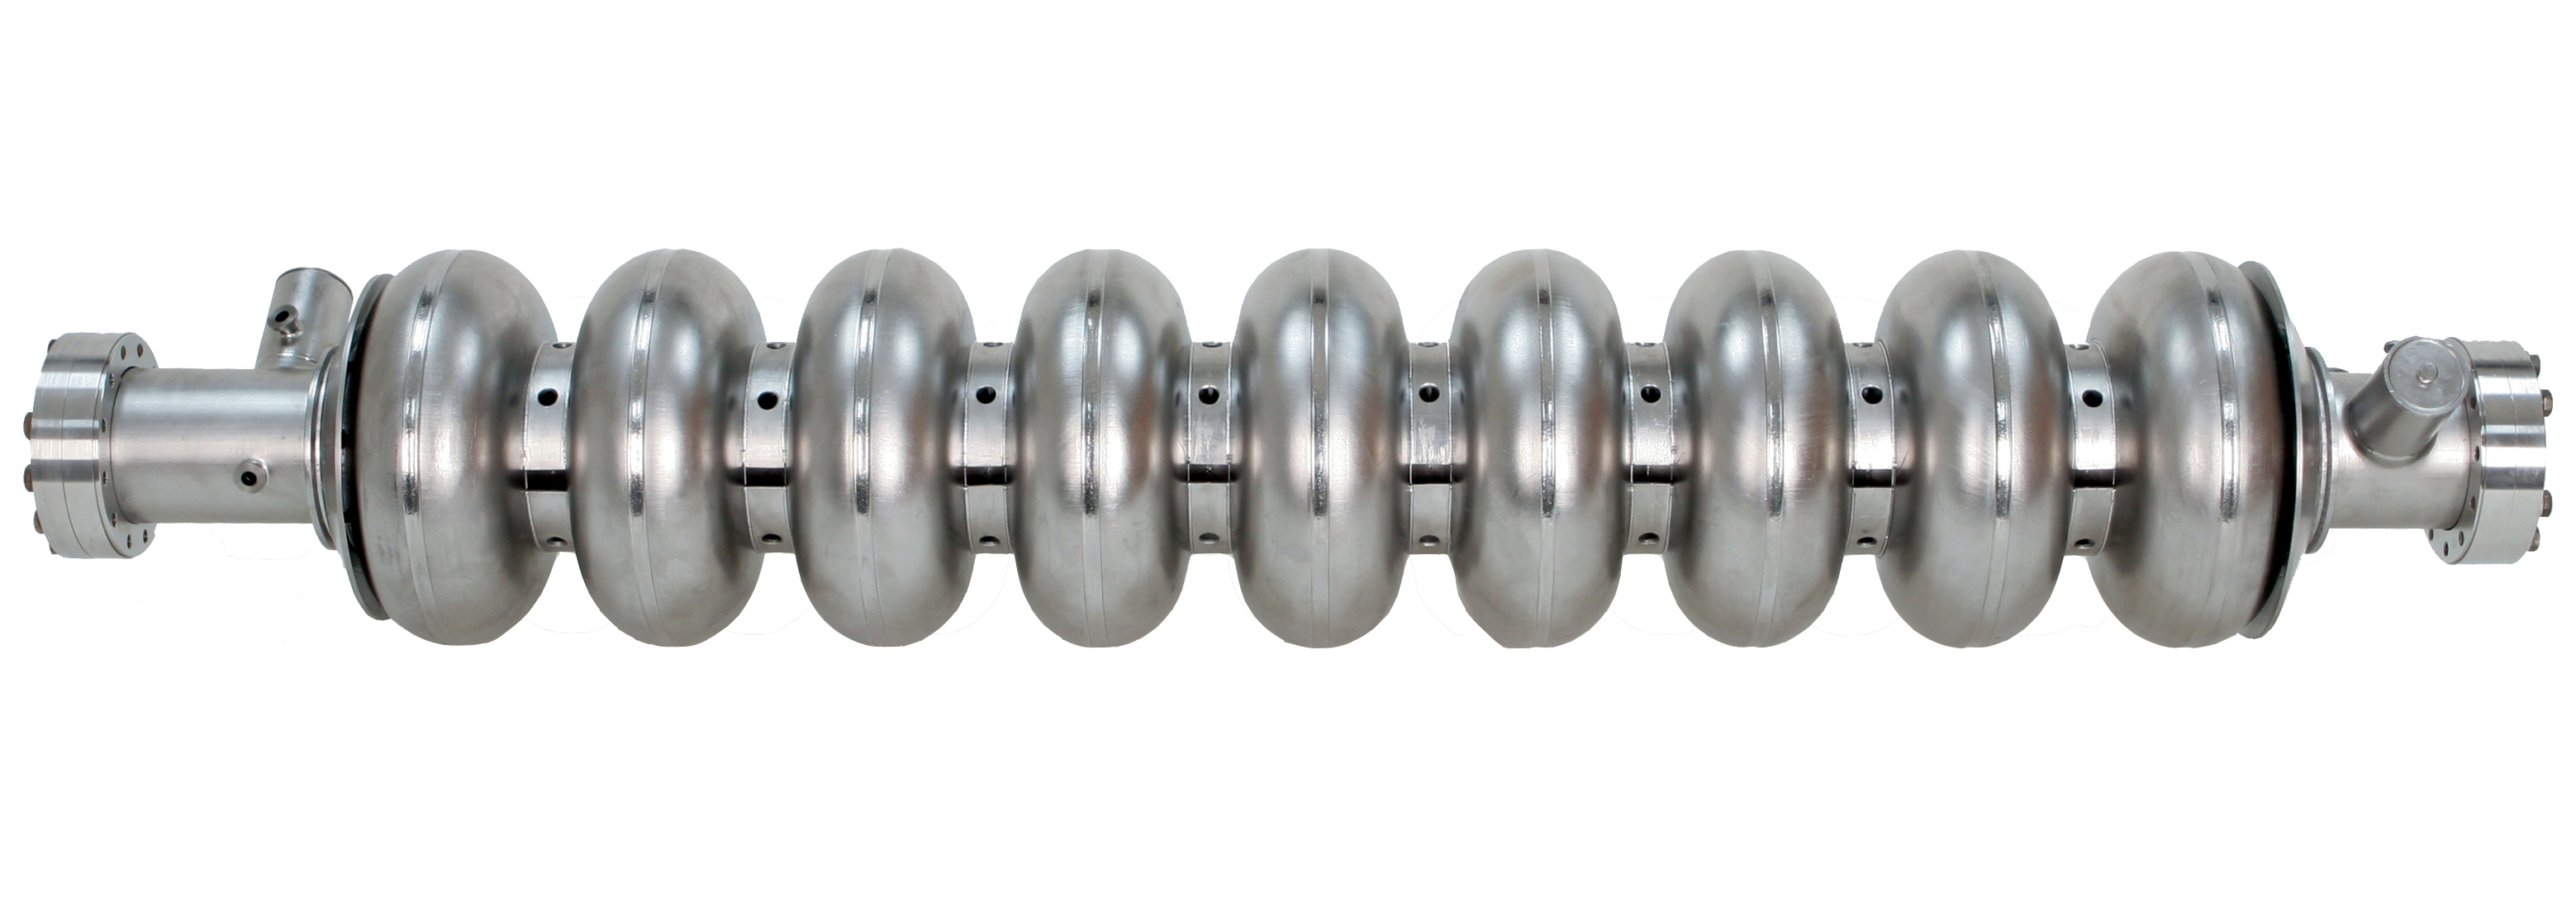
\includegraphics[width=\hsize]{chapters/figures/tesla9cell-cavity-2}
\caption{A $1.3\,{\mathrm{GHz}}$ superconducting niobium nine-cell cavity.
}
% Figure from TDR Executive Summary
% https://svnsrv.desy.de/k5websvn/wsvn/General.ilctdr/tags/FormOne-Print-Release/tdres/accel/figs/tesla9cell-cavity-2.jpg
\label{fig:tesla-cavity}
\end{figure}

After welding, the inner surface of the cavity must be prepared.
The process is designed to remove material damage incurred by chemical procedures during the fabrication process, remove chemical residues from earlier production steps, remove hydrogen in the bulk niobium from earlier chemical processing, and remove particulate contamination.
In a last step, the cavity is closed to form a hermetically sealed structure ready for transport.
The treatment steps involve a series of rinses with ethanol or high pressure water, annealing in a high purity vacuum furnace at \siunit{800^\circ}{C} and \siunit{120^\circ}{C}, and electro polishing or buffered chemical polishing.
The recipe for the surface preparation has been developed over a long time.  Still, it remains subject to optimisation, since it is a major cost driver for the cavity production and largely determines the overall performance and yield of the cavities.
In particular the electropolishing steps are complicated and costly, as they require complex infrastructure and highly toxic chemicals.
One advantage of nitrogen infusion (see Par.~\ref{par:infusion}) 
is that the final electropolishing step is omitted.

Careful quality control during the production process is of high importance.
At the European XFEL, several quality controls were conducted by the manufacturer during production, with nonconformities reported to the institute responsible for the procurement, where a decision was made whether to accept or reject a part~\cite{Singer:2016fbf}. 
With this ``build to print'' approach, in which the manufacturer guarantees that a precise production process will be followed but does not guarantee a specific performance, procurement costs are reduced, because the manufacturer does not carry, and does not charge for,  the performance risk.

Upon reception from the manufacturer, cavities are tested in a vertical cryostat (``vertical test''), where $Q_0$ is measured as a function of the gradient.
Cavities that fall below the specified gradient goal are re-treated by an additional (expensive) electropolishing step or a comparatively simple high-pressure rinse. 
After retreatment, the vertical test is repeated.

Re-treatment and tests constitute a major cost driver in cavity production. 
For the ILC TDR, it was assumed that $25\,\%$ of the cavities would fall below the \siunit{28}{MV/m} gradient threshold and undergo re-treatment and a second vertical test.
E-XFEL data from the vendor ``RI'' that followed the ILC production recipe indicate that $15\,\%$ to $37\,\%$ of the cavities fall below \siunit{28}{MV/m}, depending  on whether the maximum or the ``usable'' achieved gradient is considered~\cite{bib:Walker:2017.lcws}.
However, E-XFEL experience also shows that, in most of the cases, a high-pressure rinse is sufficient as re-treatment to remove surface defects, which is a cost saving compared to the electropolishing assumed in the TDR.

After successful testing, prior to installation in the cryomodule, cavities are equipped with a magnetic shield and the frequency tuner, which exerts mechanical force on the cavity to adjust the resonant frequency to the frequency of the external RF field~\cite[Sect. 3.3]{Adolphsen:2013kya}.  


\subsubsection{Power Coupler}

The power coupler transfers the radio frequency (RF) power from the waveguide system to the cavity. 
In the ILC, a coupler with a variable coupling is employed; this is realised using  a movable antenna.  Another role of the coupler is to 
separate the cavity vacuum from the atmospheric pressure in the waveguide, and to  insulate the cavity at \siunit{2}{K} from the surrounding room temperature.
Thus,  the coupler has to fulfill a number of demanding requirements: transmission of high RF power with minimal losses and no sparking, vacuum tightness and robustness against window breaking, and minimal heat conductivity.  
As a consequence, the coupler design is highly complex, with a large number of components and several critical high-tech manufacturing steps.

The baseline coupler design was originally developed in the 1990s for the Tesla Test Facility (TTF, now FLASH) at DESY,
and has since been modified by a collaboration of LAL and DESY for use in the European XFEL.
$800$ of these couplers (depicted in Fig. \ref{fig:xfelcoupler}) were fabricated for the European XFEL~\cite{Kaabi:2013wna} by two different companies and are now in operation.
A lot of experience has been gained from this production~\cite{Sierra:2017wyc}.



\begin{figure}[htbp]
   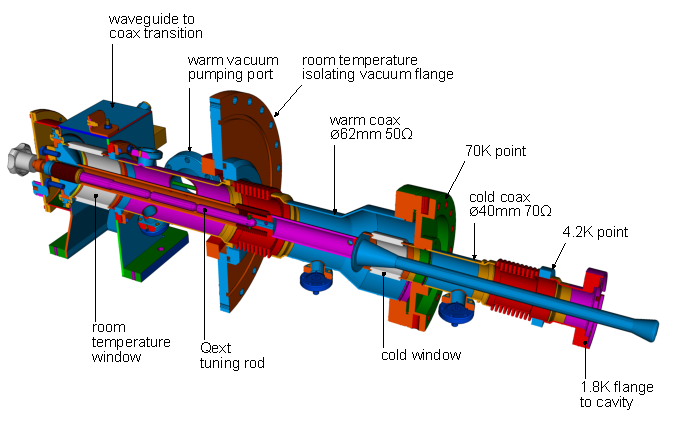
\includegraphics[width=\hsize]{chapters/figures/xfelcoupler}
\caption{An XFEL type coupler.
  % Fig from ILC TDR, should be OK to use
}
\label{fig:xfelcoupler}
\end{figure}


\subsubsection{Cryomodules}

\begin{figure}[htbp]
   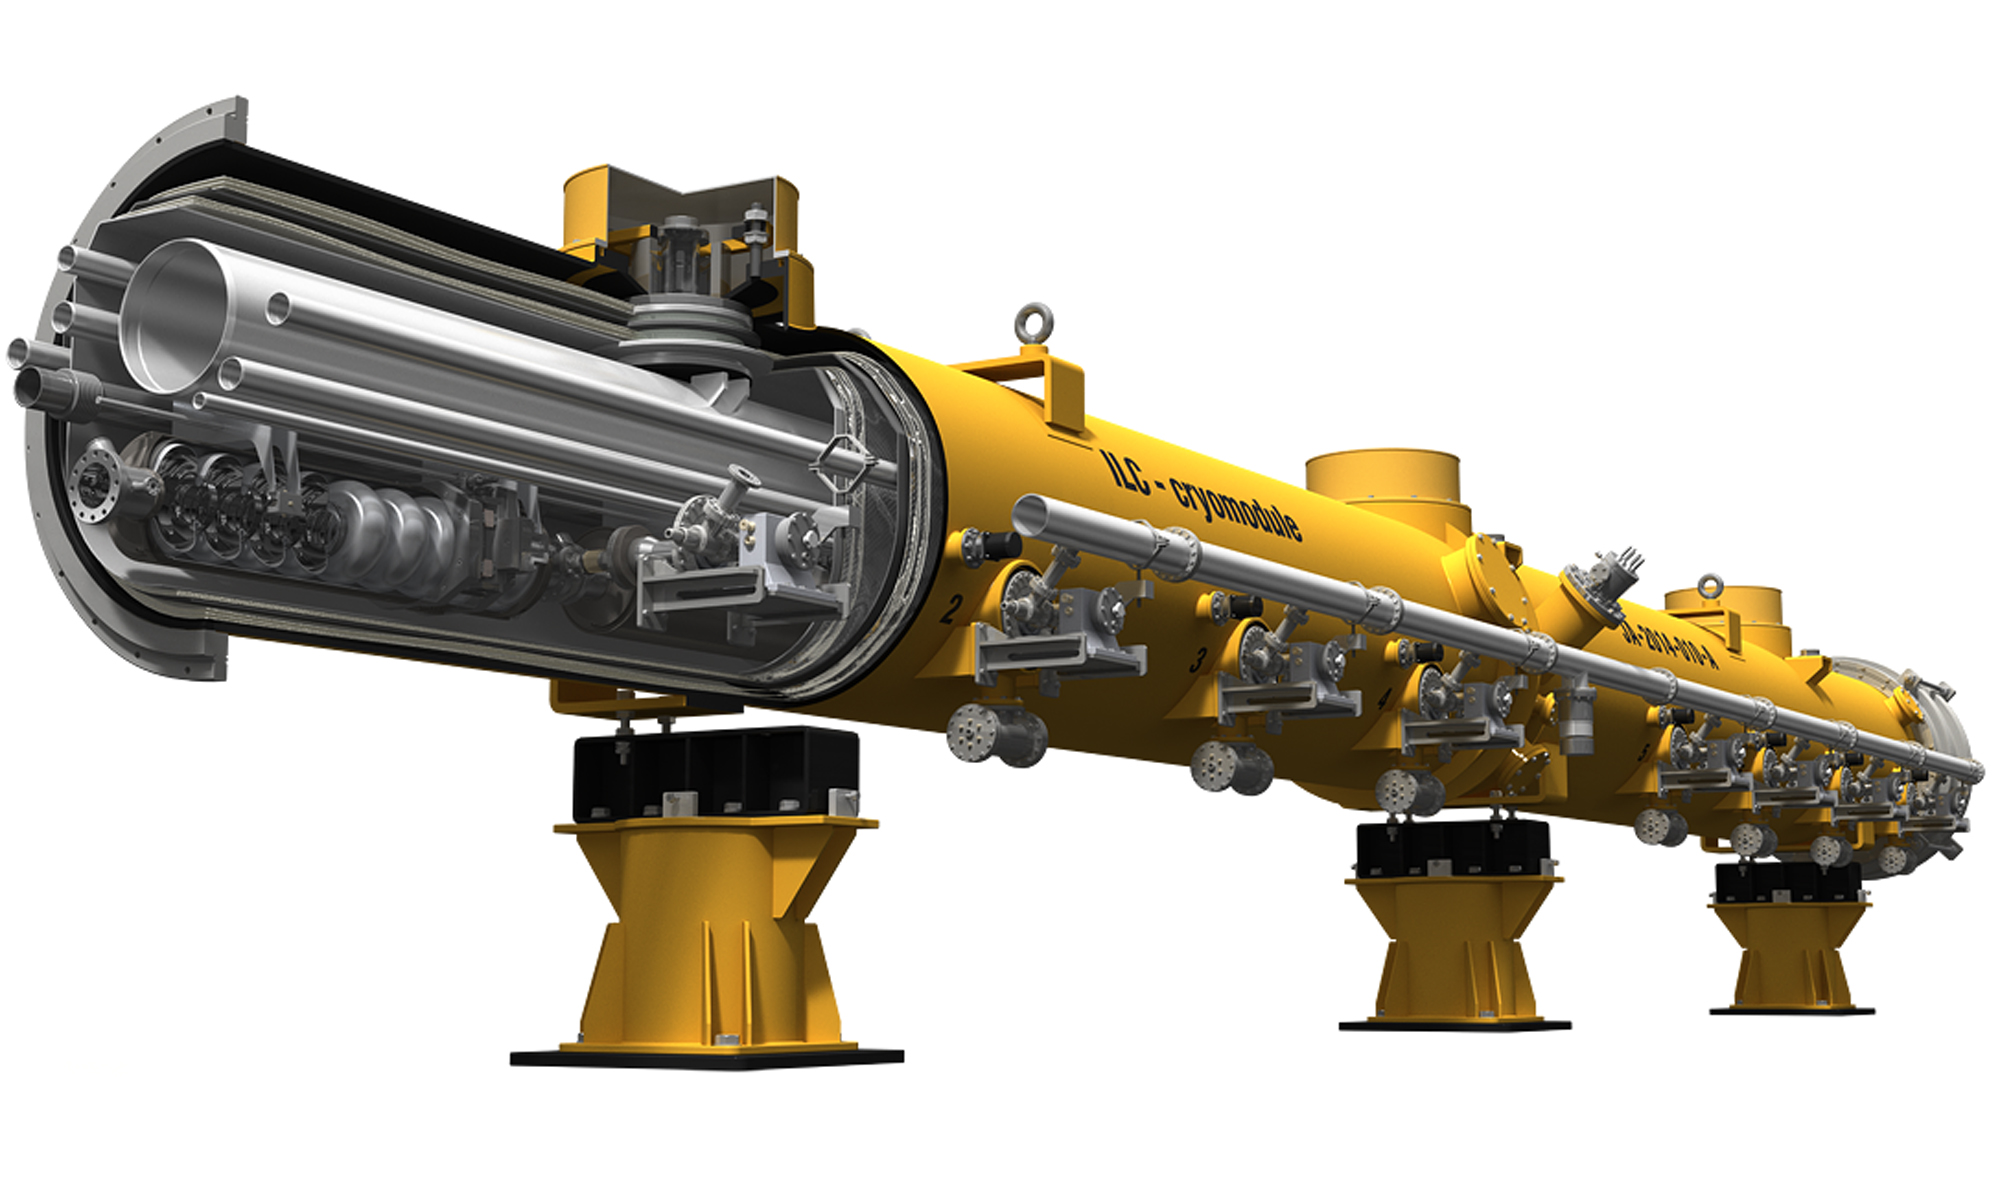
\includegraphics[width=\hsize]{chapters/figures/10_ILC_cryomodule}
\caption{An ILC type cryomodule. \copyright Rey.Hori/KEK.}
% Figure from Rey.Hori - check copyright!
% http://www.linearcollider.org/images/pid/1000890/gallery/10_ILC_cryomodule.jpg
\label{fig:crymodule}
\end{figure}

To facilitate transportation, installation and operation, 8 to 9 cavities are integrated into a \siunit{12.6}{m} long cryomodule~(Fig.~\ref{fig:crymodule}), which houses the cavities, thermal insulation, and all necessary supply tubes for liquid and gaseous helium at \siunit{2-80}{K} temperature.


\begin{figure}[htbp]
   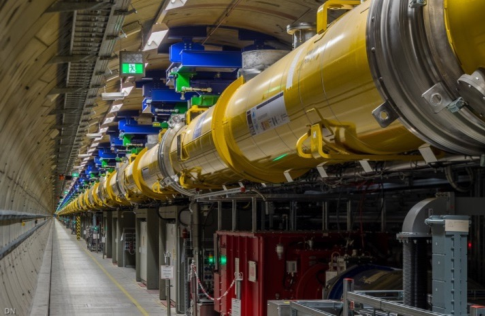
\includegraphics[width=\hsize]{chapters/figures/srf17-moxa02-fig1}
\caption{View of installed cryomodules in the tunnel of the European XFEL~\cite{Reschke:2018ywk}.
}
% Paper is published under CC-BY-3.0
\label{fig:xfel-tunnel}
\end{figure}


Nine of these cryomodules are connected in the tunnel to form a cryostring with a common liquid helium supply.  RF for one such string is provided by two klystrons.
No separate helium transfer line is necessary, as all helium transport lines are integrated within the modules.  A  quadrupole / beam position monitor / corrector magnet unit  is mounted instead of the 9th cavity in every third module.
Fig.~\ref{fig:xfel-tunnel} shows installed cryomodules in the tunnel of the European XFEL~\cite{Reschke:2018ywk}.

Cryomodule assembly requires a dedicated facility with large clean rooms, especially trained, experienced personnel, and thorough quality control~\cite{Berry:2017gpt}.
The cryomodules are certified for liquid helium pressure of up to \siunit{2}{bar}.  Thus they must  conform to the applicable pressure vessel codes, which brings with it very stringent documentation requirements for all pressure bearing parts~\cite{Peterson:2011zz}.

For the European XFEL project, 101 cryomodules were assembled by industrial partners in a dedicated facility built and operated by CEA~\cite{Weise:2014zqa,Berry:2017gpt}, demonstrating the successful industrialization of the assembly process, with a final throughput of one cryomodule every four working days.
This production rate is close to the rate envisaged for a possible European contribution of 300 cryomodules to a \siunit{250}{GeV} ILC in Japan.

\begin{figure}[htbp]
   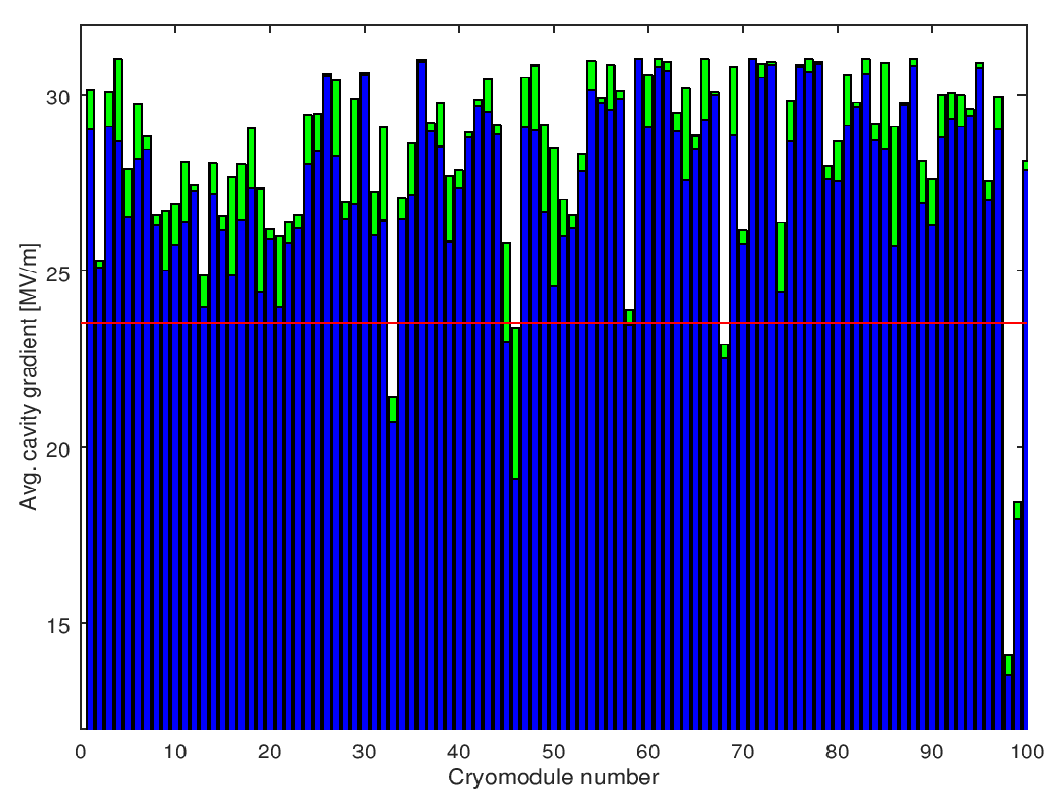
\includegraphics[width=\hsize]{chapters/figures/srf17-mopb106-fig1}
\caption{Average of the operating (blue) and maximum
(green) gradient for cavities in each European XFEL serial-production cryomodule.
The specification of \siunit{23.6}{MV/m} is marked by a red line
\cite{Kasprzak:2018kkr}.
}
% Paper is published under CC-BY-3.0
\label{fig:cryomodules-performance}
\end{figure}

While the design gradient for XFEL accelerator modules of \siunit{23.6}{MV/m} is significantly lower than the aim of \siunit{31.5-35}{MV/m} for the ILC, a number of cryomodules have been built around the world that come close or reach the ILC TDR specification of \siunit{31.5}{MV/m}: An XFEL prototype module at DESY was reached \siunit{30}{MV/m}~\cite{Kostin:2009a}, Fermilab has demonstrated cryomodule operation at the ILC specification of \siunit{31.5}{MV/m}~\cite{Broemmelsiek:2018iqr}, and KEK has reported stable pulsed operation of a cryomodule at \siunit{36}{MV/m}~\cite{Yamamoto:2018kml}.

Fig.~\ref{fig:cryomodules-performance} shows the average cavity gradients per cryomodule for the European XFEL serial-production cryomodules~\cite{Kasprzak:2018kkr}. 
For almost all of the modules, the cavity gradients are significantly above the XFEL specification of \siunit{23.6}{MV/m}.


\subsubsection{Plug-compatible design}

In order to allow various designs of sub-components from different countries and vendors to work together in the same cryomodule, a set of interface definitions has been internationally agreed upon.
This ``plug-compatible'' design ensures that components are interchangeable between modules from different regions and thus reduces the cost risk.
Corresponding interface definitions exist for the cavity, the fundamental-mode power coupler, the mechanical tuner and the helium tank.
The ``S1Global'' project~\cite{bib:s1g} has successfully built a single cryomodule from several cavities equipped with different couplers and tuners, demonstrating the viability of this concept.


\subsubsection{High-Level Radio-frequency}

The high-level radio-frequency (HLRF) system provides the RF power that drives the accelerating cavities.
The system comprises modulators, pulsed klystrons, and a waveguide power distribution system.


\paragraph{Modulators:}
The modulators provide the short, high-power electrical pulses required by the pulsed klystrons from a continuous supply of electricity. 
The ILC design foresees the use of novel, solid state Marx modulators.
These modulators are based on a solid-state switched capacitor network, where capacitors are charged in parallel over the long time between pulses, and discharged in series during the short pulse duration,
transforming continuous low-current, low voltage electricity into short high-power pulses of the required high voltage of \siunit{120}{kV} at a current of \siunit{140}{A}, over \siunit{1.65}{ms}.
Such Marx modulators have been developed at SLAC~\cite{Kemp:2011zz} 
and successfully tested at KEK~\cite{Gaudreau:2014pza}.
However, long-term data about the required large mean time between failures (MTFB) are not yet available.

\paragraph{Klystrons:}
The RF power to drive the accelerating cavities is provided by \siunit{10}{MW} L-band multi-beam klystrons. 
Devices meeting the ILC specifications were initially developed for the TESLA project, and later for the European XFEL.
They are now commercially available from two vendors (Thales and Toshiba), both of which provided klystrons for the E-XFEL.
The ILC specifications ask for a $65\,\%$ efficiency (drive beam to output RF power), which are met by the existing devices.

Recently, the High Efficiency International Klystron Activity (HEIKA) collaboration~\cite{Syratchev:2015a, Gerigk:2018ebm} has been formed that investigates novel techniques for high--efficiency klystrons.
Taking advantage of modern beam dynamic tools, methods such as the Bunching, Alignment and Collecting (BAC) method~\cite{Guzilov:2014a} and the Core Oscillation Method (COM)~\cite{Constable:2017hha} (Fig.~\ref{fig:com})
 have been developed that promise increased efficiencies up to $90\,\%$~\cite{Baikov:2015bif}.  
One advantage of these methods is that it is possible to increase the efficiency of existing klystrons by equipping them with a new electron optics, as was demonstrated retrofitting an existing tube from VDBT, Moscow. 
This increased the output power by almost 50\,\% and its efficiency from 42\,\% to 66\,\%~\cite{Jensen:2016a}.

To operate the ILC at an increased gradient of \siunit{35}{MV/m} would require that the maximum klystron output power is increased from $10$ to \siunit{11}{MW}. 
It is assumed that this will be possible by applying the results from this R\&D effort to high-efficiency klystrons.
 
\begin{figure}[htbp]
   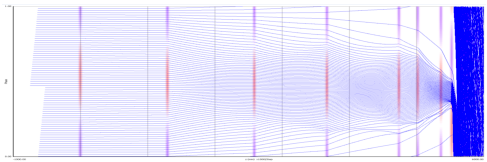
\includegraphics[width=\hsize]{chapters/figures/eefact16-wet3ah2-fig1}
\caption{Electron phase  profile of an \siunit{800}{MHz} klystron employing the Core Oscillation Method (COM)~\cite{Constable:2017hha}.
}
% Paper is published under CC-BY-3.0
\label{fig:com}
\end{figure}

\paragraph{Local Power--Distribution System (LPDS):}

In the baseline design, a single RF station with one modulator and klystron supplies RF to $39$ cavities, which corresponds to $4.5$ cryo--modules~\cite[Sec. 3.6.4]{Adolphsen:2013kya}. Then  $2$ klystrons drive a $9$ cryo--module cryo-string unit.
The power is distributed by the LPDS, a system of waveguides, power dividers and loads. 
All cavities from a $9$-cavity module and half of a $8$--cavity module are connected in one LPDS, and three such LPDS units are connected to one klystron.
This arrangement allows an easy refurbishment such that a third klystron can be added to a cryo-string, increasing the available power per cavity by $50\,\%$ for a luminosity upgrade (cf.\ Sec.~\ref{subsec:upg-opt}).

The LPDS design must provide a cost--effective solution for the  distribution of 
the RF power with minimal losses, and at the same time provide the 
flexibility to adjust the power delivered to each cavity by at least $\pm20\,\%$ to allow for 
the specified spread in maximum gradient. 
The LPDS design therefore contains remotely controlled, motor-driven Variable Power Dividers (VPD), phase shifters, and H--hybrids that can distribute the power with the required flexibility.
This design allows one to optimise the power distribution during operation, based on the cavity performance in the installed cryo--module, and thus to get the optimum performance out of the system.
It does not require a measurement of the individual cavity gradients after the module assembly, and is thus compatible with the ILC production scheme, where only a fraction of the cryo-modules are tested.
This is a notable difference from  the scheme employed at the European XFEL, where $100\,\%$ of the modules were tested, and the the power distribution for each module was tailored to the measured cavity gradients, saving investment costs for the LPDS but making the system less flexible.

\subsubsection{Cryogenics}

The operation of the large number of superconducting cryo--modules for the main linacs and the booster linacs of the sources requires a large--scale supply of liquid helium.
The cyo--modules operate at \siunit{2}{K} and are cooled with superfluid helium, which at \siunit{2}{K} has a vapour pressure of about \siunit{32}{mbar}.


The accelerator is supplied with liquid helium by several cryogenic plants~\cite[Sec. 3.5]{Adolphsen:2013kya} of a size similar to those in operation at CERN for the LHC, at Fermilab, and DESY,
with a cooling capacity equivalent to about \siunit{19}{kW} at \siunit{4.5}{K}.
The \siunit{2}{K} and \siunit{4.5}{K} helium refrigerators are located in an underground access hall~\cite{bib:cr-0014} that is connected to the surface, where the helium compressors, gas tanks and further cryogenic infrastructure are located.
The total helium inventory is approximately $310 000$ liquid litres or about $41$ metric tonnes, about one third of the LHC's helium inventory.  A factor 2 more helium is needed for 
500~GeV operation.


%\subsubsection{Existing and Future Facilities}

% XXXXX MORE HERE  XXXXXXXX

\subsubsection{Series Production and Industrialisation, Worldwide and in Europe}

Due to the construction of the European XFEL, the industrial basis for the key SCRF components is broad and mature, in particular in Europe.
Europe has a leading supplier for raw material. 
In all three regions (Europe, America, Asia), several vendors for cavities have been qualified for ILC type cavities, and provided cost estimates in the past.
Two leading cavity vendors are European companies that have profited from large scale production of cavities for XFEL; 
both have won contracts for LCLS-II as a consequence, which illustrates the potential to create revenue from outside Europe should the ILC be built.
RF couplers have also been successfully produced by European and  American vendors for the XFEL and LCLS-II projects.

ILC/TESLA type cryo modules have been built in laboratories around the world (DESY, CEA in Europe, FNAL and JLAB in America, KEK in Asia).
Series production has been established in America at Fermilab and JLAB for LCLS-II,.
The largest series production was conducted by CEA in France, again for the XFEL, with the assembly of \num{103} cryo modules in total by an industrial partner under the supervision of CEA personnel, with a final throughput of one cryo module produced every four working days.

ILC type, pulsed \siunit{10}{MW} klystrons are commercially available from two vendors in Japan and Europe.

For XFEL, China has been a supplier for niobium raw material and cryomodule cold masses (the cryostat with internal insulation and tubing).
For the planned SCLF project in Shanghai, China has started to develop cavity and cryo module production capabilities, which will further broaden the worldwide production capabilities for SCRF components.
This reduces the risk that prices are pushed up by a monopoly of manufacturers for a large scale order of components as required for the iLC.

Overall, European industry is well prepared to produce the high-tech, high-value SCRF components needed for the ILC, which would likely constitute largest fraction of any European in-kind contribution (IKC) to the ILC, at very competitive prices.
Thus, expenditure for the European IKC will likely stay in Europe, with an excellent chance to stay within the price range assumed in the value estimate.
Moreover, European companies are well poised to win additional contracts from other regions, increasing the economic benefit for Europe from an ILC project.



%===============================================================================

\subsection{Accelerator Design}

\subsubsection{Electron and Positron Sources}

The electron and positron sources are designed to produce \siunit{5}{GeV} beam pulses with a bunch charge that is $50\,\%$ higher than the design bunch charge of \siunit{3.2}{nC} ($\siunit{2\cdot 10^{10}}{e}$), in order to have sufficient reserve to compensate  any unforeseen inefficiencies in the beam transport.
In the baseline design, both sources produce polarized beams with the same time structure as the main beam, \ie, $1312$ bunches in a $\siunit{727}{\mu s}$ long pulse.

The electron source design~\cite{Adolphsen:2013kya} is based on the SLC polarized electron source, which has demonstarted that the bunch charge, polarisation and cathode lifetime parameters are feasible.
The long bunch trains of the ILC do require a newly developed laser system and powerful preaccelerator structures, for which preliminary designs are available.
The design calls for  a Ti:sapphire laser impinging on a photocathode based on a strained GaAs/GaAsP superlattice
structure, which will produce electron bunches with an expected polarisation of \siunit{85}{\%},
sufficient for \siunit{80}{\%} beam polarization at the interaction point, as demonstrated at SLAC~\cite{Alley:1995ia}.

The positron source poses a larger challenge. 

In the baseline design, hard gamma rays are produced in a helical undulator driven by the main electron beam, which are converted to positrons in a rotating target.
Positrons are captured in a flux concentrator or a quarter wave transformer, accelerated to \siunit{400}{MeV} in two normal conducting preaccelerators followed by a superconducting accelerator very similar to the main linac, before they are injected into the damping rings at \siunit{5}{GeV}.
Compared to planar undulators, the helical undulators produce twice as many photons, and with circular polarisation, which is transferred to the positrons produced in the target.
The positron polarisation thus achieved is $30\,\%$.
The E-166 experiment at SLAC has successfully demonstrated this concept  \cite{Alexander:2009nb}, albeit at intensities much lower than foreseen for the ILC. 
Technological challenges of the undulator source concept are the target heat load, the radiation load in the flux concentrator device, and the dumping of 
the high intensity photon beam remnant.

As an alternative, an electron-driven positron source concept has been developed.
In the electron-driven scheme, a \siunit{3}{GeV} electron beam from a dedicated normal conducting linac produces positrons in a rotating target.
The electron drive beam, being independent from the main linac, has a completely different time structure. 
Positrons are produced in $20$ pulses at \siunit{300}{Hz} with $66$ bunches each.  With this scheme, it takes about \siunit{67}{ms} to produce the  positrons needed for a single Main Linac pulse with its $1312$ bunches, compared to \siunit{0.8}{ms} for the undulator source.
This different time structure spreads the heat load on the target over a longer time, allowing a target rotation speed of only \siunit{5}{m/s} rather than \siunit{100}{m/s}, which reduces the engineering complexity of the target design, in particular the vacuum seals of the rotating parts.
Although not free from its own engineering challenges, such as the high beam loading in the normal conducting cavities, the electron driven design is currently considered to be a low risk design that is sure to work.

Aside from the low technical risk, the main advantage of the electron driven design is the independence of positron production and electron main linac operation, which is an advantage for accelerator commissioning and operation in general.
In particular, electron beam energies below \siunit{120}{GeV} for operation at the $Z$ resonance or the $WW$ threshold would be no problem.
The undulator source, on the other hand, offers the possibility to provide beams at the maximum repetition rate of \siunit{10}{Hz} given by the damping time in the damping rings of \siunit{100}{ms}, whereas the electron driven scheme is limited to \siunit{6}{Hz} due to the additional \siunit{66}{ms} for positron production.
The main difference between the concepts is the positron polarisation offered by the undulator source, which adds significantly to the physics capabilities of the machine.  The physics implications of positron polarization is discussed later in the report, in Secs.~\ref{subsec:beampol} and {subsec:polarisation}. 

Both concepts have been reviewed recently \cite{PWG:2018a} inside the ILC community, with the result that both source concepts appear viable, with no known show stoppers, but they
require some more engineering work. 
The decision on the choice will be taken once the project has been approved, based on the physics requirements, operational aspects, and technological maturity and risks. 

\paragraph{Beam polarisation and spin reversal}
\label{par:beampol}

At the ILC, the electron beam and potentially the positron beam are longitudinally polarised at the source, \ie,  the polarisation vector is oriented parallel or antiparallel 
to the beam direction.
Whenever a longitudinally polarised beam of energy $E\sub{beam}$ is deflected by an angle $\theta\sub{bend}$, the polarisation vector undergoes a BMT precession though through an angle $\theta\sub{pol} =  \gamma a \theta\sub{bend}$~\cite{Moffeit:2005pb}, 
with the Lorentz factor $\gamma = E\sub{beam}/m\sub{e}$ and the electron's anomalous magnetic moment $a = (g-2)/2$. 
To preserve the longitudinal beam polarisation during the long transport from the source through the damping rings to the start of the main linac, which involves many horizontal bends, the beam polarisation vector is rotated into the transverse plane, perpendicular to the damping ring plane, before the beam is transferred to the damping rings, and rotated back to a longitudinal direction by a set of spin rotators at the end of the RTML (see Sec.~\ref{sec:rtml}).
Through the use of two rotators, it is possible to bring the polarisation vector into any desired direction, and compensate any remaining net precession between these spin rotators and the interaction point, so that any desired longitudinal or transverse polarisation at the IP can be provided.

To control systematic effects, fast helicity reversal is required.  This is helicity reversal of each beam independently, on a pulse to pulse basis, which must be achieved without a change of the magnetic fields of the spin rotator magnets.
For the electron beam, a fast helicity reversal is possible through a flip of the cathode laser polarisation.  For the undulator-based positron source, the photon polarisation is given by the undulator field.  Two parallel sets of spin rotators in front of the damping rings are used that rotate the polarisation vector either to the $+y$ or $-y$ direction.  With this scheme,
fast kickers can select a path through either of the two spin rotators and thus provide a fast spin reversal capability~\cite{Moffeit:2005pb,Malysheva:2016jdr}.




\subsubsection{Damping Rings}

The ILC includes two oval damping rings of \siunit{3.2}{km} circumference, sharing a common tunnel in the central accelerator complex.
The damping rings reduce the horizontal and vertical emittance of the beams by almost six orders of magnitude\footnote{The vertical emittance of the positrons is reduced from $\epsilon_{\mathrm{y}} \approx 0.8\,{\mathrm{\mu m}}$ to $2\,{\mathrm{pm}}$.} within a time span of only \siunit{100}{ms}, to provide the low emittance beams required at the interaction point. 
Both damping rings operate at an energy of \siunit{5}{GeV}.

The damping rings' main objectives are
\begin{itemize} 
\item to accept electron and positron beams at large emittance and produce the low-emittance beams required for high-luminosity production,
\item to dampen the incoming beam jitter to provide highly stable beams,
\item to 
delay bunches from the source to allow feed-forward systems to compensate for pulse-to-pulse variations in parameters such as the bunch charge.
\end{itemize}

Compared to today's fourth generation light sources, the target value for the normalized beam emittance ($\siunit{4}{\mu m}$/\siunit{20}{nm} for the normalised horizontal / vertical beam emittance) is low, but not a record value, and it is thus considered to be a realistic goal.

The main challenges for the damping ring design are to provide
\begin{itemize} 
\item a sufficient dynamic aperture to cope with the large injected emittance of the positrons,
\item a low equilibrium emittance in the horizontal plane,
\item a very low emittance in the vertical plane,
\item a small damping time constant,
\item damping of instabilities from electron clouds (for the positron DR) and fast ions (for the electron DR),
\item a small (\siunit{3.2-6.4}{ns}) bunch spacing, requiring very fast kickers for injection and ejection.
\end{itemize}

Careful optimization has resulted in a TME (Theoretical Minimum Emittance) style lattice for the arcs that balances a low horizontal emittance with the required large dynamic aperture~\cite[Chap. 6]{Adolphsen:2013kya}. 
Recently, the horizontal emittance has been reduced further by lowering the dispersion in the arcs through the use of longer dipoles~\cite{bib:cr-0016}.
The emittance in the vertical plane is minimised by careful alignment of the magnets and tuning of the closed orbit to compensate for misalignments and field errors, as demonstrated at the CESRTA accelerator~\cite{Billing:2011zc}.

The required small damping time constant requires large synchrotron radiation damping, which is provided by the insertion of $54$ wigglers in each ring.
This results in an energy loss of up to $7.7\,{\mathrm{MV}}$ per turn and up to $3.3\,{\mathrm{MW}}$ RF power to 
store the positron beam at the design current of $390\,{\mathrm{mA}}$.  This
actually exceeds the average beam power of the accelerated positron beam, $2.6\,{\mathrm{MW}}$ at 
a $250\,{\mathrm{GeV}}$.

Electron cloud (EC) and fast ion (FI) instabilities limit the overall current in the damping rings to about \siunit{400-800}{mA}, where the EC limit that affects the positrons is assumed to be more stringent. 
These instabilities arise from electrons and ions being attracted by the circulating beam towards the beam axis. 
A low base vacuum pressure of \siunit{10^{-7}}{Pa} is required to limit these effects to the required level.
In addition, gaps between bunch trains of around $50$ bunches are required in the DR filling pattern, which permits the use of clearing electrodes to mitigate EC formation.
These techniques have been developed and tested at the CESR-TA facility~\cite{Conway:2012zza}

In the damping rings, the bunch separation is only \siunit{6.4}{ns} (\siunit{3.2}{ns} for a luminosity upgrade to $2625$ bunches). 
Extracting individual bunches without affecting their emittance requires kickers with rise/fall times of \siunit{3}{ns} or less.
Such systems have been tested at ATF~\cite{Naito:2010zzb}.

The damping ring RF system will employ superconducting cavities operating at half the Main Linac frequency (\siunit{650}{MHz}).
Klystrons and accelerator modules can be scaled from existing \siunit{500}{MHz} units in operation at CESR and KEK~\cite[Sec. 6.6]{Adolphsen:2013kya}. 


\subsubsection{Low Emittance Beam Transport: Ring to Main Linac (RTML)}
\label{sec:rtml}

The Ring to Main Linac (RTML) system~\cite[Chap. 7]{Adolphsen:2013kya} is responsible for transporting and matching the beam from the Damping Ring to the entrance of the Main Linac.
Its main objectives are
\begin{itemize} 
\item transport of the beams from the Damping Rings at the center of the accelerator complex to the upstream ends of the Main Linacs,
\item collimation of the beam halo generated in the Damping Rings,
\item rotation of the spin polarisation vector from the vertical to the desired angle at the IP (typically, in longitudinal direction).
\end{itemize}

The RTML consists of two arms for the positrons and the electrons. 
Each arm comprises a damping ring extraction line transferring the beams from the damping ring extraction into the main linac tunnel, a long low emittance transfer line (LTL), the turnaround section at the upstream end of each accelerator arm, and a spin rotation and diagnostics section.

The long transport line is the largest, most costly part of the RTML.
The main challenge is to transport the low emittance beam at \siunit{5}{GeV} with minimal emittance increase, and in a cost-effective manner, considering that its total length is about \siunit{14}{km} for the \siunit{250}{GeV} machine.

In order to preserve the polarisation of the particles generated in the sources, their spins are rotated into a vertical direction (perpendicular to the Damping Ring plane) before injection into the Damping Rings. 
A set of two rotators~\cite{Emma:1995kf} employing superconducting solenoids allows to rotate the spin into any direction required.

At the end of the RTML, after the spin rotation section and before injection into the bunch compressors (which are considered part of the Main Linac, not the RTML~\cite{bib:cr-0010}), a diagnostics section allows measurement of  the emittance and the  coupling between the  horizontal and vertical plane.
A skew quadrupole system is included to correct for any such coupling.

A number of circular fixed-aperture and rectangular variable-aperture collimators in the RTML provide betatron collimation at the beginning of the LTL, in the turn around and before the bunch compressors.


\subsubsection{Bunch Compressors and Main Linac}

\begin{figure}[htbp]
   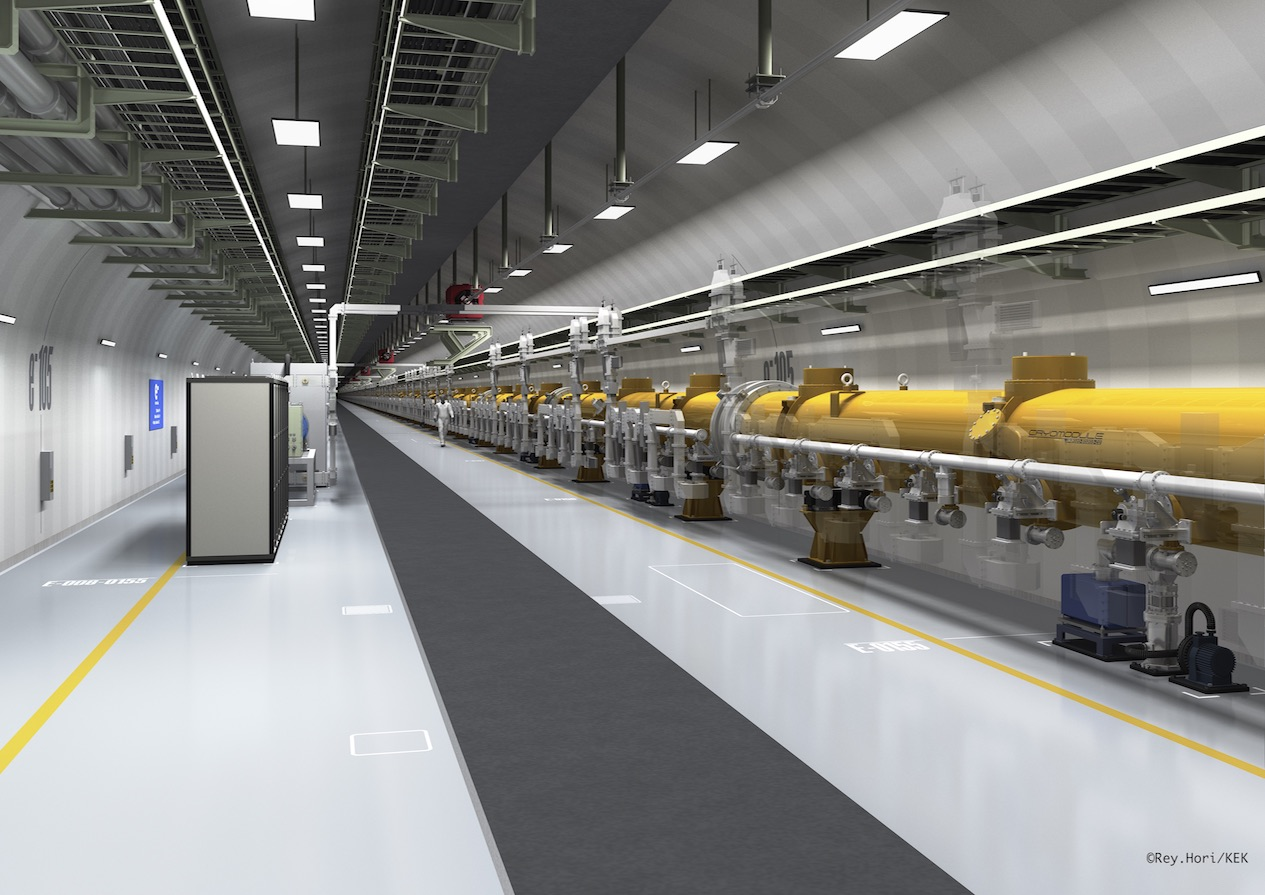
\includegraphics[width=\hsize]{chapters/figures/ILC2016_tunnel_A1_160826-low4}
\caption{Artist's rendition of the ILC Main Linac tunnel. The shield wall in the middle has been removed.
\copyright Rey.Hori/KEK.}
\label{fig:ilc-tunnel}
\end{figure}

The heart of the ILC are the two Main Linacs, which accelerate the beams from $5$ to \siunit{125}{GeV}.
The linac tunnel, as depicted in Figs.~\ref{fig:ilc-tunnel} and \ref{fig:ml-tunnel}, has two parts, separated by a shield wall. 
One side (on the right in Fig.~\ref{fig:ilc-tunnel}) houses the beamline with the accelerating cryomodules as well as the RTML beamline hanging on the ceiling.
The other side contains power supplies, control electronics, and the modulators and klystrons of the High-Level RF system.
The concrete shield wall (indicated as a dark-grey strip in in Fig.~\ref{fig:ilc-tunnel}) has a thickness of \siunit{1.5}{m}~\cite{bib:cr-0012}.
The shield wall allows access to the electronics, klystrons and modulators during operation of the klystrons with cold, resonant cavities, protecting personnel from X-ray radiation emanating from the cavities caused by dark currents.
Access during beam operation, which would require a wall thickness of \siunit{3.5}{m}, is not possible.

\begin{figure}[htbp]
   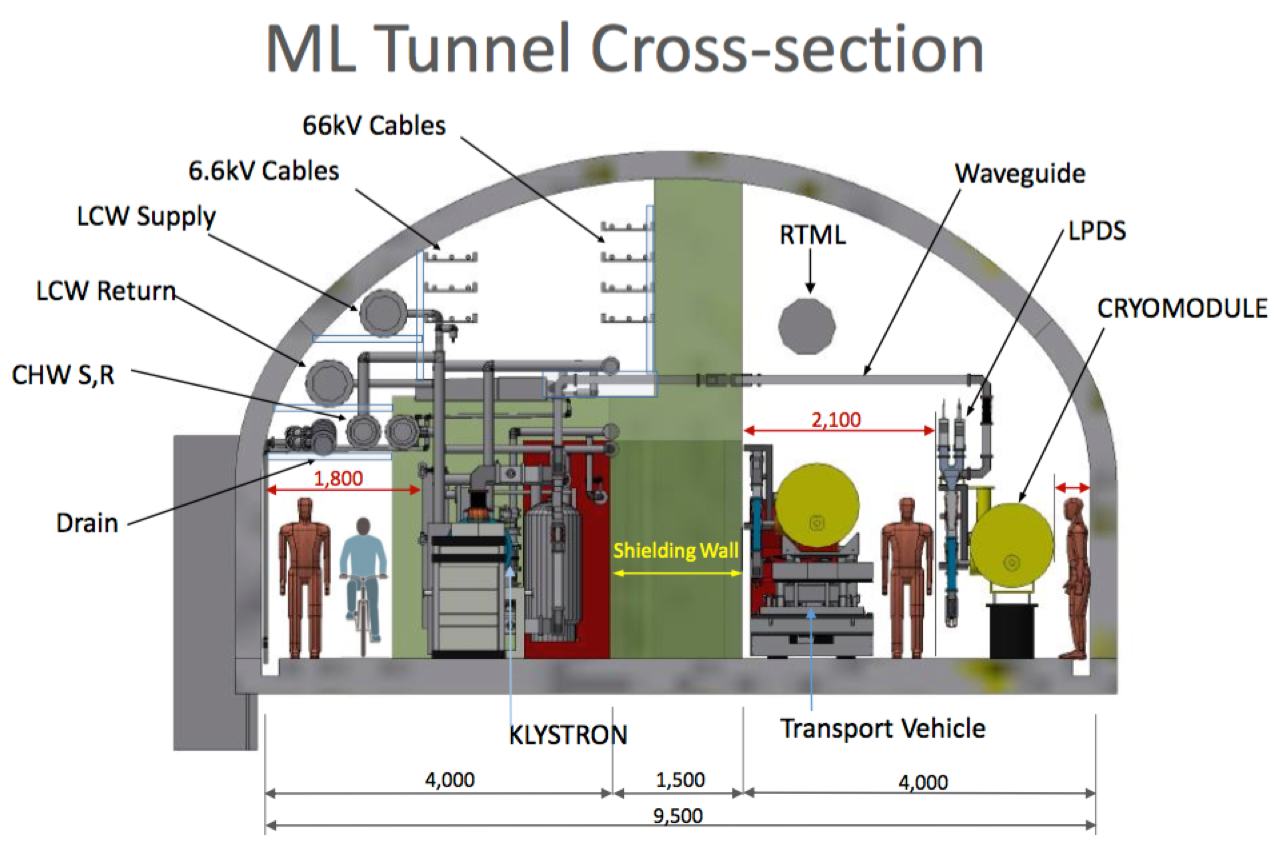
\includegraphics[width=\hsize]{chapters/figures/ML-cross-section}
\caption{Cross section through the Main Linac tunnel.}
\label{fig:ml-tunnel}
\end{figure}

The first part of the Main Linac is a two-stage bunch compressor system~\cite[Sec. 7.3.3.5]{Adolphsen:2013kya}, each consisting of an accelerating section followed by a wiggler. 
The first stage operates at \siunit{5}{GeV}, with no net acceleration, the second stage accelerates the beam to \siunit{15}{GeV}.
The bunch compressors reduce the bunch length from $6$ to \siunit{0.3}{mm}.

After the bunch compressors, the Main Linac continues for about \siunit{6}{km} with four long strings of cryomodules. 

\paragraph{RF distribution:}

Each \siunit{12.65}{m} long cryomodule contains $9$ cavities, or for every third module, $8$ cavities and a package with a superconducting quadrupole, corrector magnets, and beam position monitor.
Nine such modules, with a total of $117$ cavities, are powered by $2$ klystrons and provide 3.83 (4.29)~\GeV at a gradient of \siunit{31.5 (35)}{MV/m}.
The waveguide distribution system allows an easy refurbishment to connect a third klystron for a luminosity upgrade.
The $50\,\%$ RF power increase would allow $50\,\%$ higher current through smaller bunch separation, and longer beam pulses because of a reduced filling time, so that the number of bunches per pulse and hence the luminosity can be doubled, while the RF pulse duration of \siunit{1.65}{ms} stays constant.

\paragraph{Cryogenic supply:}


Each $9$ module unit \siunit{114}{m} long, forms a cryo string, which is connected to the helium supply line with a Joule-Thomson valve.
All helium lines are part of the cryomodule, obliterating the need for a separate helium transfer line. 
Up to $21$ strings with $189$ modules and \siunit{2.4}{km} total length can be connected to a single plant; 
this is limited by practical plant sizes and the gas--return header pressure drop.  


\paragraph{Cost reduction from larger gradients:}

Fig.~\ref{fig:ml-cryo-opta} shows the layout of the cryogenic supply system for the \siunit{250}{GeV} machine.
At the top, the situation is depicted for the gradient of \siunit{31.5}{MV/m} with a quality factor of $Q\sub{0}=1.0\cdot 10^{10}$, as assumed in the TDR~\cite{Adolphsen:2013kya}. 
In this case, the access points PM$\pm 10$ would house two cryogenic plants, each supplying up to $189$ cryomodules or an equivalent cryogenic load.
The bottom picture shows the situation for a gradient of \siunit{35}{MV/m} with $Q\sub{0}=1.6\cdot 10^{10}$, as could be expected from successful R\&D. 
The increased gradient would  allow reduction of the total number of cryomodules by roughly $10\,\%$ from $987$ to $906$. The increased quality factor would reduce the dynamic losses such that $4$ cryo plants would provide sufficient helium. In the top configuration $6$ large plants in the access halls plus $2$ smaller plants in the central region would be needed.

In all of these ways, the accelerator is designed to make good use of any anticipated performance gain from continued high gradient R\&D,  in the case that raising the gradient is
seen to be  beneficial from an economical point of view, without incurring unwanted technology risk.

\begin{figure}[htbp]
   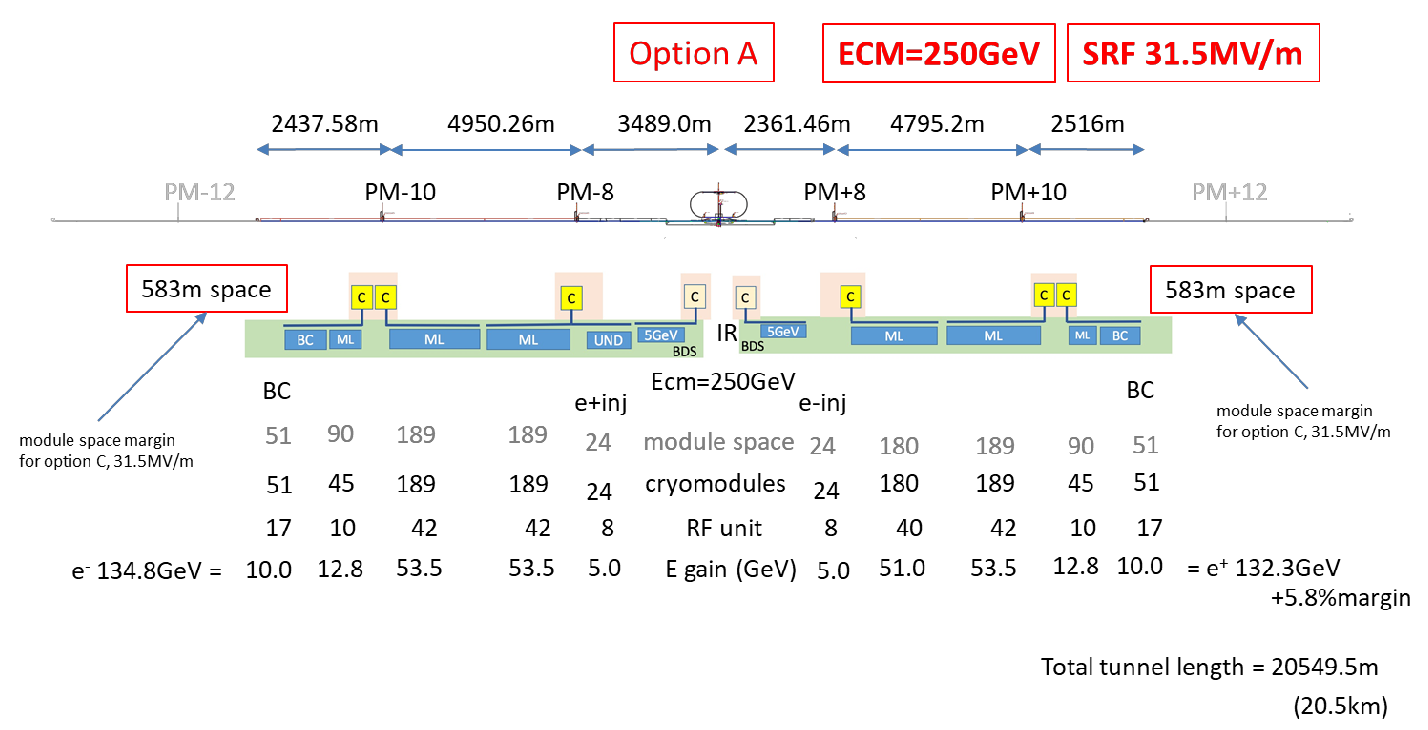
\includegraphics[width=\hsize]{chapters/figures/arxiv-1711-00568-fig-3-4}
   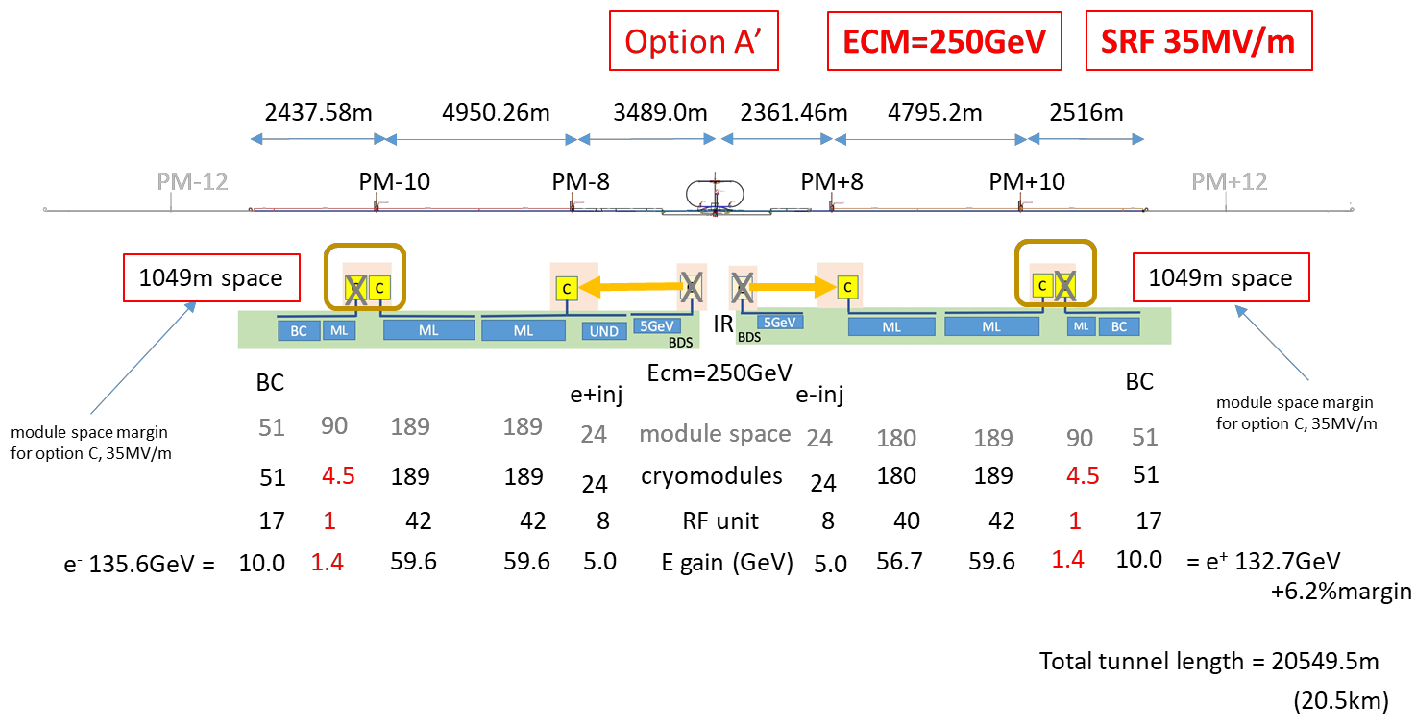
\includegraphics[width=\hsize]{chapters/figures/arxiv-1711-00568-fig-3-7}
\caption{Cryogenic layout for a gradient of \siunit{31.5}{MV/m} (top) and \siunit{35}{MV/m} (bottom)~\cite{Evans:2017rvt}.
``Module space'' indicates how many cryomodules can be physically installed, ``cryomodules'' and ``RF unit'' indicates the number of actually installed modules and klystrons (one klystron per 4.5 cryomodules). ``E gain'' indicates the energy gain in GeV. ``BC'', ``ML'', ``e+ inj'', ``e- inj'' and ``UND'' refer to the sections with need for liquid helium: bunch compressor, main linac, 5GeV boosters in the positron and electron source, and the positron source undulator section, respectively. PM$\pm8, 10, 12$ refer to access hall locations, ``C'' to cryo plants; meter numbers on top indicate the length of the corresponding section.}
\label{fig:ml-cryo-opta}
\end{figure}



\subsubsection{Beam Delivery System and Machine Detector Interface}

The Beam Delivery System (BDS) transports the $e^+/e^-$ beams from the end of the main linacs, focuses them to the required small beam spot at the Interaction Point (IP), brings them into collision, and transports the spent beams to the main dumps~\cite[Chap. 8]{Adolphsen:2013kya}.
The main functions of the BDS are
\begin{itemize}
\item measuring the main linac beam and matching it into the final focus,
\item protecting beamline and detector from mis-steered beams~\footnote{On the electron side, the protective fast beam abort system is actually located upstream of the positron source undulator.},
\item remove large amplitude (beam--halo) and off--momentum particles from the beam to minimize background in the detector,
\item accurately measure the key parameters energy and polarisation before and after the collisions.
\end{itemize}
The BDS must provide sufficient diagnostic and feedback systems to achieve these goals.

The BDS is designed such that it can be upgraded to a maximum beam energy of \siunit{500}{GeV}; components such as the dumps that are not cost drivers for the overall project but would be cumbersome to replace later are dimensioned for the maximum beam energy from the beginning.
In other places, such as the energy collimation dogleg, those components necessary for \siunit{125}{GeV} beam operation are installed and space for a later upgrade is reserved.

Overall, the BDS is \siunit{2254}{m} long from the end of the main linac (or the undulator and target bypass insert of the positron source on the electron side, respectively) to the IP.

\paragraph{Diagnostics and collimation section:}
The BDS starts with a diagnostics section, where emittance, energy and polarisation are measured and any coupling between the vertical and horizontal planes is corrected by a set of skew quadrupoles.
The energy measurement is incorporated into the machine protection system and can, \eg,  extract off-momentum bunches caused by a klystron failure in the main linac that would otherwise damage the machine or detector.
An emergency dump~\cite{bib:cr-0013} is dimensioned such that it can absorb a full beam pulse at \siunit{500}{GeV}, sufficient for \siunit{1}{TeV} operation.

The diagnostics section is followed by a collimation system, which first removes beam halo particles (betatron collimation). 
Then, off-momentum particles are removed.
In this energy collimation section, sufficient dispersion must be generated by bending the beam in a dogleg, while avoiding excessive synchrotron radiation generation in dispersive regions that leads to an increase of the horizontal emittance.
This emittance dilution effect grows as $E\sub{beam}^6$ at constant bending radius for the normalised emittance, and determines the overall length of the energy collimation section for a maximum \siunit{500}{GeV} beam energy to about \siunit{400}{m}.


\paragraph {Final focus with feedback system and crab cavities:}
\label{par:final_focus}

The final focus system demagnifies the beam to the required spot size of \siunit{516 \times 7.7}{nm^2} by means of a final quadrupole doublet.
Even the relatively small energy spread of $\approx 0.1\,\%$ leads to a significant spread of the focal length of the doublet and requires a correction to achieve the desired beam size, which is realised by a local chromaticity correction scheme~\cite{Raimondi:2000cx}.

To bring the beams to collision with the neccessary nanometre accuracy requires a continuous compensation of drift and vibration effects.
Along the ILC, the pulse length and bunch separation (\siunit{727}{\mu s} and \siunit{554}{ns}, respectively) are large enough to allow corrections between pulses as well as within a bunch train (intratrain feedback).
Beam-beam offsets of a fraction of the beam size lead to a measurable deflection of the outgoing beams,and these measurements are used to feed fast stripline kickers that stabilize the beam.
\siunit{3.9}{GHz} crab cavities close to the interaction point are incorporated that rotate the bunches to compensate for the \siunit{14}{mrad} beam crossing angle~\cite[Sect. 8.9]{Adolphsen:2013kya}.
 

\paragraph {Test results from ATF2:}
The Accelerator Test Facility 2 (ATF2) was built at KEK in 2008 as a test bed for the ILC final focus scheme~\cite[Sec. 3.6]{Adolphsen:2013jya}.
Its primary goals were~\cite{Grishanov:2005ek,Grishanov:2006kx} to achieve a \siunit{37}{nm} vertical beam size at the interaction point (IP), and to demonstrate beam stabilisation at the nanometre level.
After scaling for the different beam energies (ATF2 operates at $E\sub{beam}=\siunit{1.3}{GeV}$), the \siunit{37}{nm} beam size corresponds to the TDR design value of $\sigma\sub{y}^* = \siunit{5.7}{nm}$ at \siunit{250}{GeV} beam energy.
As Fig.~\ref{fig:atf-results} shows, this goal has been reached within $10\,\%$~\cite{Okugi:2017jji} by the successive application of various correction and stabilisation techniques, 
validating the final focus design, in particular the local chromaticity correction~\cite{White:2014vwa}.

The fifth generation FONT5 feedback system~\cite{Apsimon:2018bpq} for the ILC and CLIC has also been tested at the ATF2, where a beam stabilisation to \siunit{41}{nm} has been demonstrated~\cite{Ramjiawan:2018egu}.

\begin{figure}[htbp]
   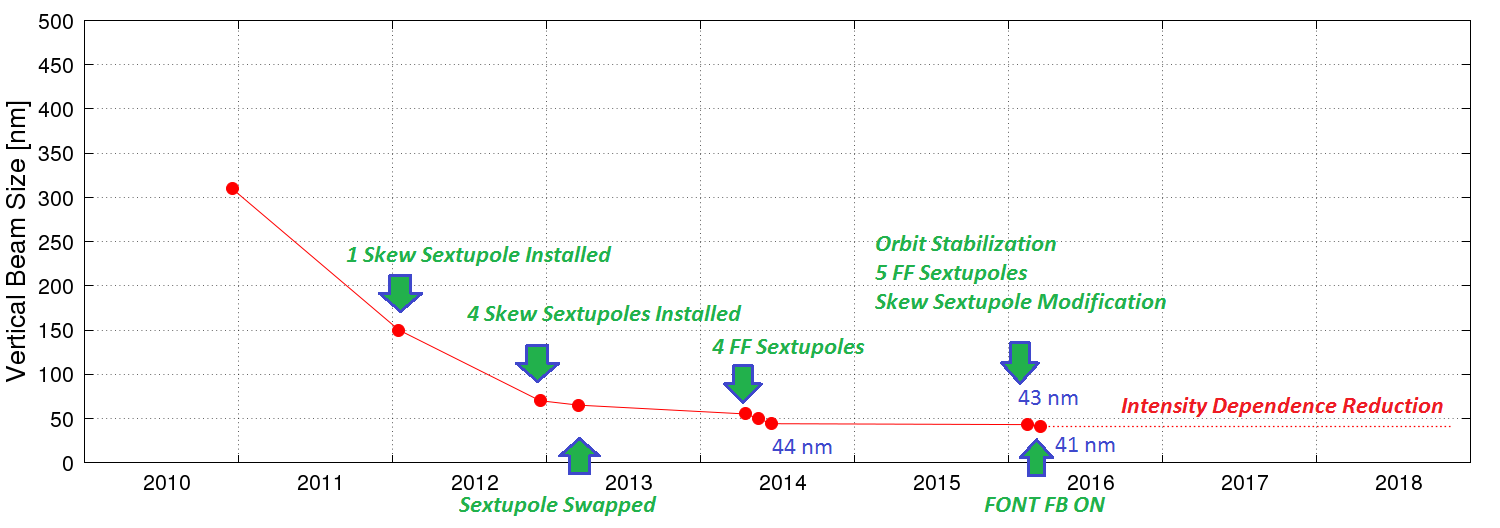
\includegraphics[width=\hsize]{chapters/figures/ATF2trend2018}
\caption{Beamsizes achieved at the Accelerator Test Facility 2 (ATF2) as a function of time~\cite{bib:atf2esu}. The latest result (\siunit{41}{nm}~\cite{Okugi:2017jji}) is within $10\,\%$ of the goal beam size of \siunit{37}{nm}.}
\label{fig:atf-results}
\end{figure}

\paragraph {Machine detector interface (MDI):}

% describe experimental hall, final focus

% XXXXXXXXXXXXX BEGIN NEW 20190219 XXXXXXXXXXXXXX

The ILC is configured to have two detectors that share one interaction point, with one detector in data taking position at any time, in a so--called ``push--pull'' operation~\cite[Sec. 8.4]{Adolphsen:2013jya}.
Both detectors are mounted on movable platforms that allow an exchange of the detectors within approximately \siunit{24}{hours}.

In the push--pull scheme, the innermost final focus quadrupole ``QD0'', a slim, superconducting magnet package combined with a sextupole for lacal chromaticity correction, is installed within the detectors. 
The other part of the final focus doublet (``QF1'') is located outside the detector on a bridge, and does not move with the detector.
Since the TDR, the free space $L^*$ between interaction point and the QD0 edge has been harmonised to a common value of $L^*=\siunit{3.5}{m}$~\cite{bib:cr-0002}, which facilitates the design of a final focus optics that delievers optimal and equal performance to both detectors.

The detectors are located in an underground cavern. 
In contrast to the TDR design, it is foreseen to have a large vertical access shaft~\cite{bib:cr-0003}, which permits a CMS--style detector installation concept, in which the detectors are assembled in large modules in a surface hall and lowered into the hall by means of a gantry crane capable of lowering pieces up to \siunit{4000}{t}.
As the CMS experience shows, this concept significantly reduces the schedule risk associated with the experimental hall, as it the cavern needs to be available for detector installation only one or two years prior to commissioning.

% \paragraph {Extraction line}

% XXXXXXXXXXXXX END NEW 20190219 XXXXXXXXXXXXXX

\paragraph {Main dump:}

The main beam dumps~\cite[Sect. 8.8]{Adolphsen:2013kya} are rated for a maximum beam power of \siunit{17}{MW}~\cite{bib:cr-0013}, enough for a \siunit{1}{TeV} upgrade of the accelerator.
The main dump design is based on the successful SLAC \siunit{2.2}{MW} beam dump~\cite{Walz:1967nz}.
It  utilises water at \siunit{10}{bar} pressure (to prevent boiling) as absorber medium. 
The main engineering challenges lie in the safe recombination of the produced oxyhydrogen gas and in the safe containment and disposal of radioisotopes, in particular tritium and $^7{\mathrm{Be}}$ produced from spallation processes.
The entry window is another component that has to be carefully designed. 

% XXXXXXXXXXXXX BEGIN NEW 20190219 XXXXXXXXXXXXXX

\paragraph {Measurement of beam energy, luminosity, and beam polarisation:}

Two energy spectrometers, one located \siunit{700}{m} upstream of the IP, the other \siunit{55}{m} downstream, provide independent and complementary measurements of the beam energy with an accuracy of \siunit{100}{ppm}~\cite{Boogert:2009ir}.

The luminosity is measured to $10^{-3}$ accuracy from low angle Bhabha scattering in the so--called LumiCal (see Sect.~\ref{susub:det:forward}) at polar angles from $30$ to \siunit{90}{mrad}.
Additional calorimeters (BeamCal) in the region $5$ to \siunit{30}{mrad} provide a fast signal that is used to detect beam--beam offsets of a fraction of the beam size, and correct them via the intra--beam feedback system (see Par.~\ref{par:final_focus}).

Beam polarisation is measured with \siunit{0.25}{\%} accuracy by means of Compton scattering: electrons that scatter off green or infrared light laser photons lose enough energy that they can be detected in a spectrometer; their momentum spectrum is used to fit the beam polarisation~ \cite{Vormwald:2015hla}.
Two such polarimeters are located \siunit{1800}{m} upstream and \siunit{150}{m} downstream of the IP, which allows to interpolate the precise polarisation at the IP and control the systematics, including effects from precession of the polarisation vector by transverse fields and depolarising effects in the interaction, which lead to a sizeable variation of the polarisation within the bunch during the collision (see Sect.~\ref{subsubsec:sysuncert}). 


% XXXXXXXXXXXXX END NEW 20190219 XXXXXXXXXXXXXX


%===============================================================================

\subsection{Upgrade Options \label{subsec:upg-opt}}

Given the high initial investment for a facility as large as the ILC, it is mandatory to have an interesting physics programme for several decades, with the possibility to adapt the programme to the needs arising from the knowledge obtained by the LHC, the ILC itself, all other particle physics experiments, and other branches of physics such as cosmology.
Several options exist for upgrades of the ILC in terms of energy, luminosity, and beam polarisation.

\subsubsection{Energy upgrade}
\label{subsubsec:upg-optE}

The obvious advantage of a linear collider is its upgradeability in energy.
Basically, the main linacs can be extended as far as desired, at constant cost per added beam energy, with some added cost for the relocation of the turn arounds and bunch compressors.
Additional costs arise when the beam delivery system (BDS), including the beam dumps, has to be extended to handle the increased beam anergy; 
the current ILC BDS is designed to be easily upgradeable for centre of mass energies up to \siunit{1}{TeV} at minimal cost.

Depending on the actual gradient achieved for the construction of the ILC, there may be space for the installation of up to $171$ additional cryomodules, which would increase the centre-of-mass energy by about \siunit{54}{GeV} to around \siunit{304}{GeV}, as Fig.~\ref{fig:ml-cryo-opta} shows, 
and possibly require the installation of two additional cryo plants.

A further energy upgrade would require extension of the tunnel.
The Kitakami site can accommodate a total accelerator length of at least \siunit{50}{km}, more than enough for a \siunit{1}{TeV} centre--of--mass energy.
Any extension of the accelerator would proceed by adding new cryomodules at the low energy (upstream) ends of the accelerator, there is no need to move modules already installed. 

An upgrade would likely proceed in two phases: a preparation phase while the accelerator is still operated and produces data, and a refurbishment phase where the accelerator is shut down.

During the preparation phase, the necessary components---in particular the cryomodules, klystrons, and modulators---would be acquired and built.
At the same time, civil engineering would proceed with the excavation of new access tunnels, underground halls, and the main tunnel.
Recent studies conducted during road tunnel construction in the Kitakami area, in the same rock formation as foreseen for the ILC, indicate that the level of vibrations caused by tunnelling activities would allow to bring the new tunnels quite close to the existing ones before machine operation would be affected~\cite{bib:sanuki:lcws2018}, minimising the shutdown time necessary.

During the installation phase, the newly built tunnels would be connected to the existing ones, the beam lines at the turn-around and the wiggler sections of the bunch compressors would be dismantled, and the new cryomodules would be installed as well as the new turn-around and bunch compressors. 
At the same time, any necessary modifications to the positron source and the final focus can be made.
With the cryo modules ready for installation at the beginning of the shut down period, it is estimated that the shutdown could be limited to about a year for an energy upgrade.

% {\it XXXXXXXX Mention quantization from timing constraint, leads to stage with 500-600 GeV, optimal for tth and testing Higgs self coupling in the region relevant for electroweak baryogenesis Sec. \ref{subsubsec:runscen_ilc500} XXXXXXXX }

\subsubsection{Luminosity upgrade}
\label{subsubsec:upg-optL}

The luminosity of the ILC can be increased by increasing the luminosity per bunch (or per colliding charge), or increasing the number of bunches per second~\cite{Harrison:2013nva}.

Increasing the luminosity per bunch requires a smaller beam spot size, which may be achieved by tighter focusing and/or smaller beam emittance.
Studies indicate that with enough operating experience, there is potential for a further luminosity increase. 
This route to increased luminosity is, however, invariably linked to higher beam disruption, which brings larger energy spread and higher backgrounds and thus more challenging conditions for the experiments.

The ILC design also has the potential to increase the number of colliding bunches per second, by doubling the number of bunches per pulse, and possibly by increasing the pulse repetition frequency.

Doubling the number of bunches per pulse to $2625$ would require a smaller bunch spacing, requiring  the installation of $50\,\%$ more klystrons and modulators. 
Since  the RF pulse length of \siunit{1.65}{ms} is unchanged, the cryogenic load is essentially unchanged.
Doubling the number of bunches would double the beam current in the damping rings.
For the positron damping ring, this may surpass the limitations from electron cloud (EC) instabilities. 
To mitigate this risk, the damping ring tunnel is large enough to house a third damping ring, so that the positron current could be distributed over two rings.

The pulse repetition rate (\siunit{5}{Hz} in the baseline configuration) is limited by the available cryogenic capacity, the damping time in the damping rings, and the target heat load in the positron source target.
The damping rings are designed for a \siunit{100}{ms} damping time and thus capable of a repetition rate of up to \siunit{10}{Hz}, twice the nominal rate.
Operation at an increased repetition rate would be possible if after an energy upgrade the machine is operated below its maximum energy (e.g., \siunit{250}{GeV} operation of a \siunit{500}{GeV} machine for a larger low-energy data set), or if additional cryogenic capacity is installed.

\subsubsection{Polarisation upgrade}
\label{subsubsec:upg-optP}

The baseline design foresees at least $80\,\%$ electron polarisation at the IP, combined with $30\,\%$ positron polarisation for the undulator positron source.
At beam energies above \siunit{125}{GeV}, the undulator photon flux increases rapidly. 
Photons polarisation is maximal at zero emission angle; it is decreased and even inverted at larger angles.
Thus, collimating the surplus photon flux at larger emission angles increases the net polarisation. 
Studies indicate that $60\,\%$ positron polarisation at the IP may be possible at \siunit{500}{GeV} centre--of--mass energy with the addition of a photon collimator.
 


%===============================================================================

\subsection{Civil Engineering and Site}


In 2014, the ILC Strategy Council announced the result of its candidate site evaluation for the best possible ILC site in Japan~\cite{ILCSC:2014a}.
The evaluation was conducted by a number of Japanese experts from universities and industry, and reviewed by an international commitee. 
It considered technical as well as socio-environmental aspects, and concluded that the candidate site in the Kitakami region is best suited for the ILC.

\begin{figure}[htbp]
   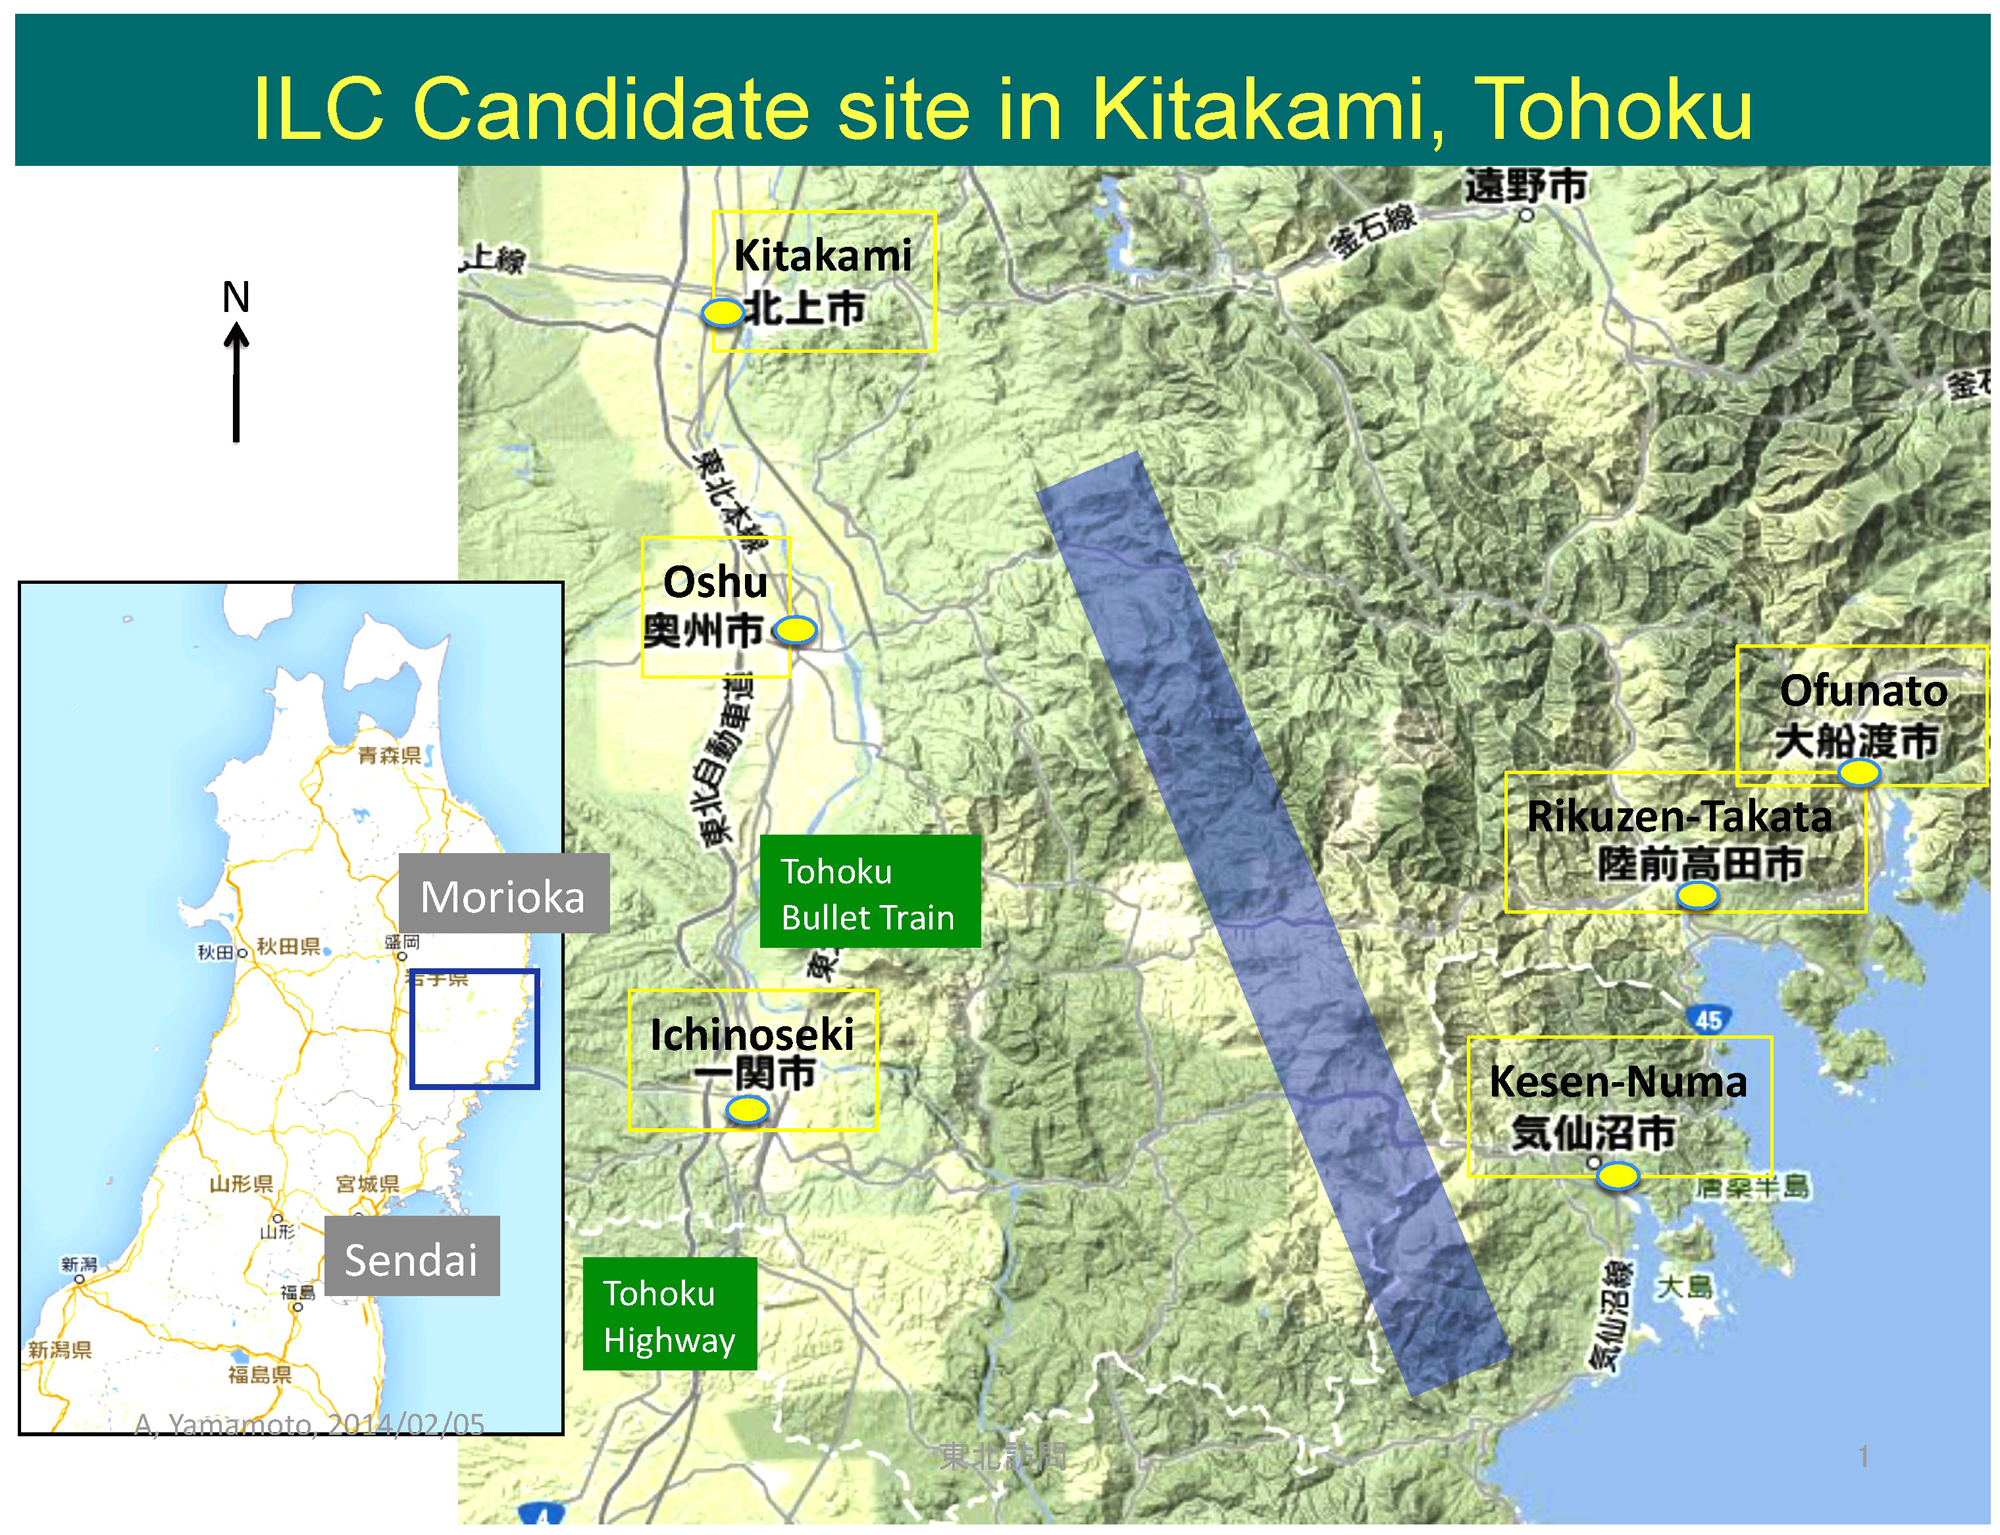
\includegraphics[width=\hsize]{chapters/figures/ILC-Candidate-Area2}
\caption{The Kitakami candidate site for the ILC~\cite{Warmbein:2014a}.}
\label{fig:kitakami-site}
\end{figure}

The site (Fig.~\ref{fig:kitakami-site}) is located in the Japan's northern Tohoku region, not far from Sendai with its international airport, in the prefectures of Iwate and Miyagi.
The closest cities are Ichinoseki, Oshu, and Kitakami, which all offer Shinkansen (bullet train) access to Sendai and Tokyo.
The closest harbour is in the city of Kesen-Numa.
The coastal region in this area was severely hit by the great Tohoku earthquake in 2011. 
Both prefectures are supportive of the ILC project and view it as an important part of their strategy to recover from the earthquake disaster.

The Kitakami site was largely selected because of its excellent geological condition. 
The proposed ILC trajectory lies in two large, homogeneous granite formations, the Hitokabe granite in the north and Senmaya granite to the south.
The site provides up to \siunit{50}{km} of space, enough for a possible \siunit{1}{TeV} upgrade or more, depending on the achievable accelerating gradient.  
Extensive geological surveys have been conducted in the area, including boring, seismic measurements, and electrical measurements~\cite{Sanuki:2015a}, as shown in Fig.~\ref{fig:kitakami-geology}.
The surveys show that the rock is of good quality, with no active seismic faults in the area.

Earthquakes are frequent throughout Japan, and the accelerator and detectors need  proper supports that isolate them from vibrations during earthquakes and micro tremors~\cite{Sanuki:2018b}. 
Proven technologies exist to cope with all seismic events, including magnitude 9 earthquakes such as the great Tohoku earthquake. 

% XXXXX MENTION TUNNELLING TECHNOLOGY (NAT), Cross section, Tomo's talk on earthquake vibes XXXXXXXX

Vibration measurements taken during the construction of a road tunnel show that accelerator operation would be possible during the excavation of a tunnel for an energy upgrade~\cite{Sanuki:2018a}.


% XXXXXXX CONTINUE HERE XXXXXXXXXX

\begin{figure}[htbp]
   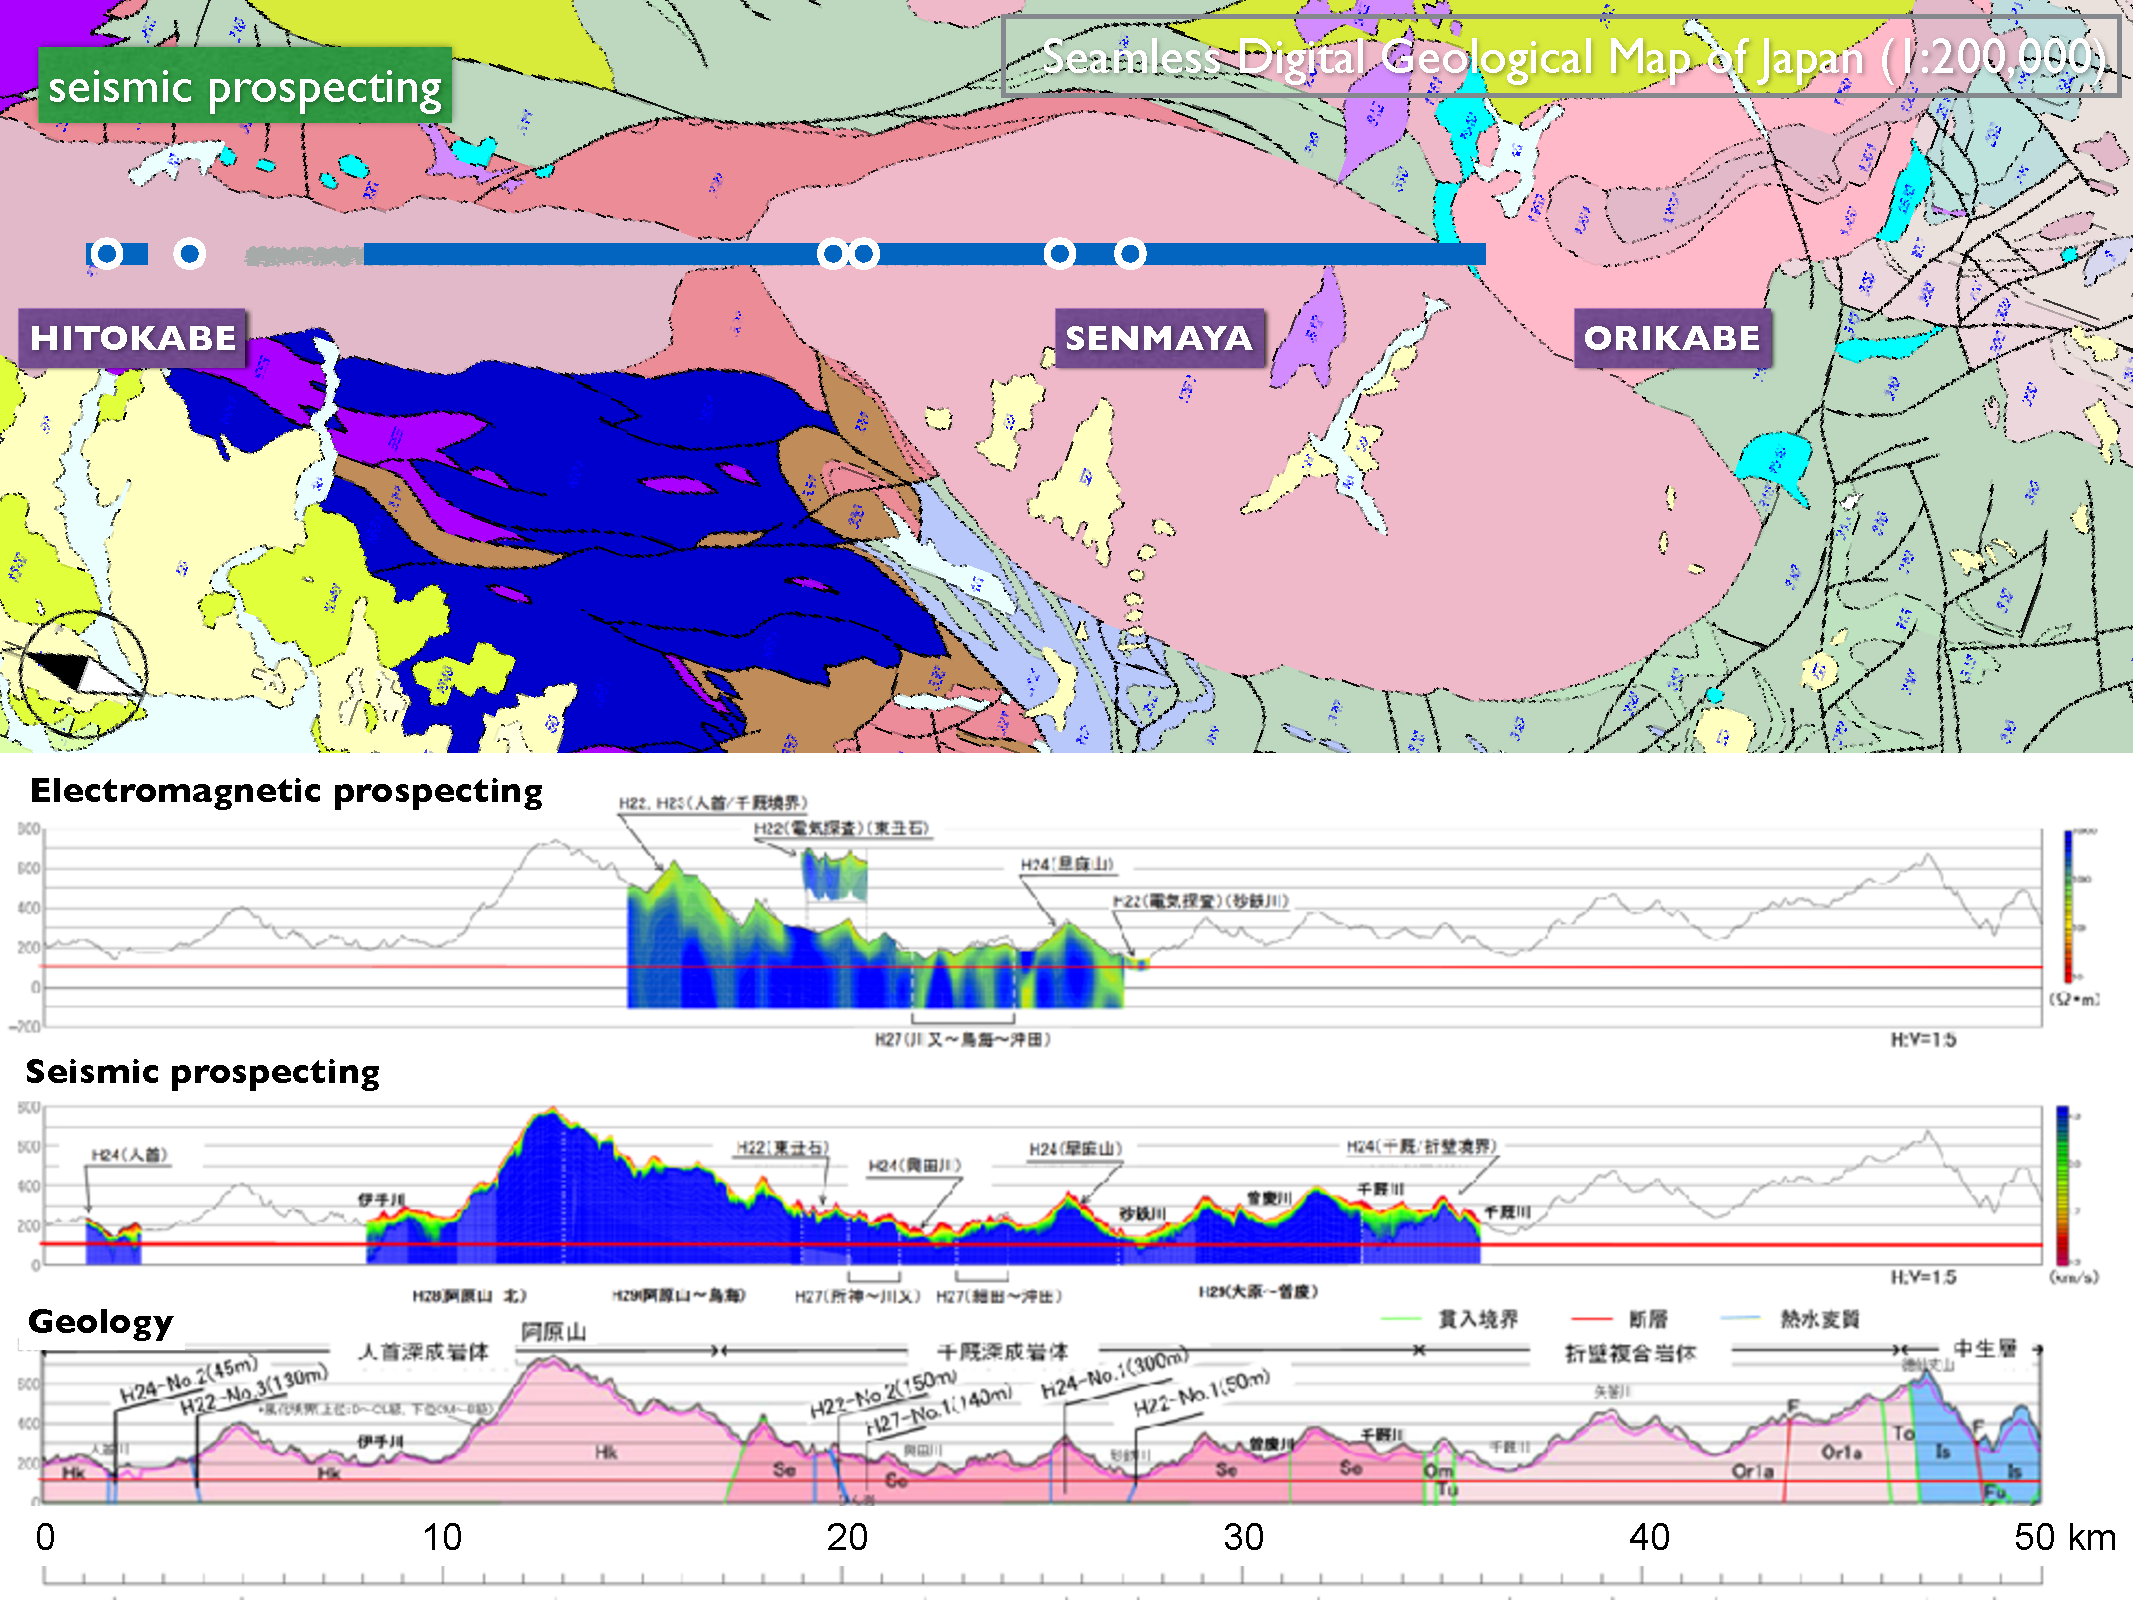
\includegraphics[width=\hsize]{chapters/figures/Kitakami_Geology}
\caption{Geological situation at the Kitakami site.}
\label{fig:kitakami-geology}
\end{figure}


%===============================================================================

\begin{figure*}[htbp]
 %\epsfysize=9.0cm
 \begin{center}
 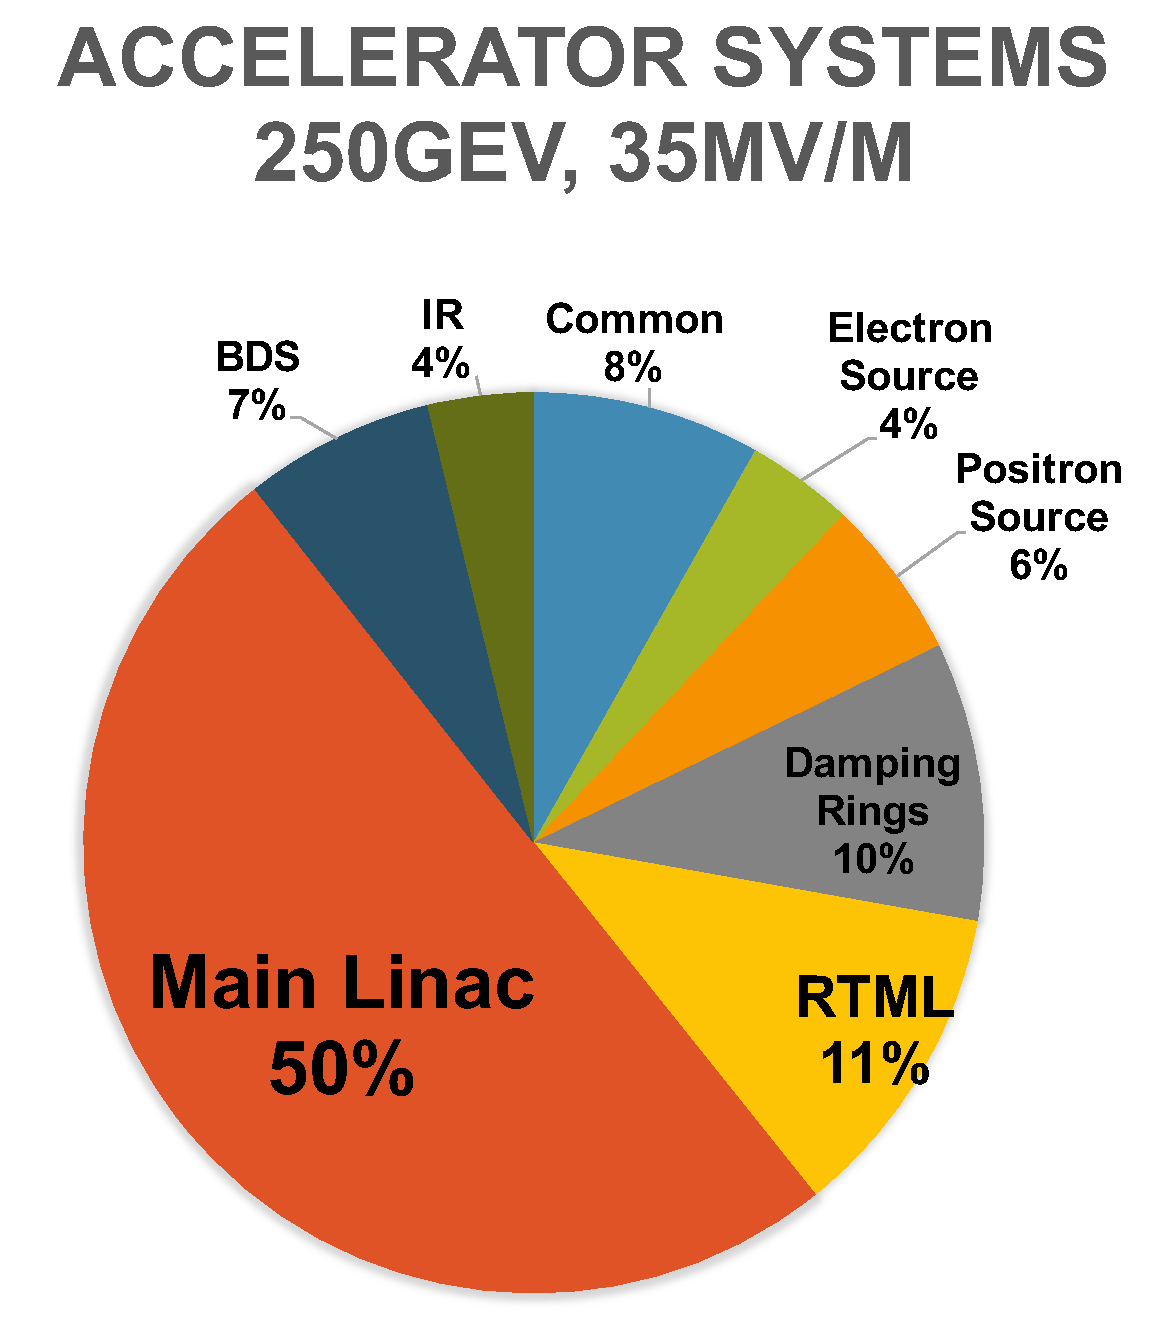
\includegraphics[width=0.36\hsize]{chapters/figures/costs-as.pdf}
 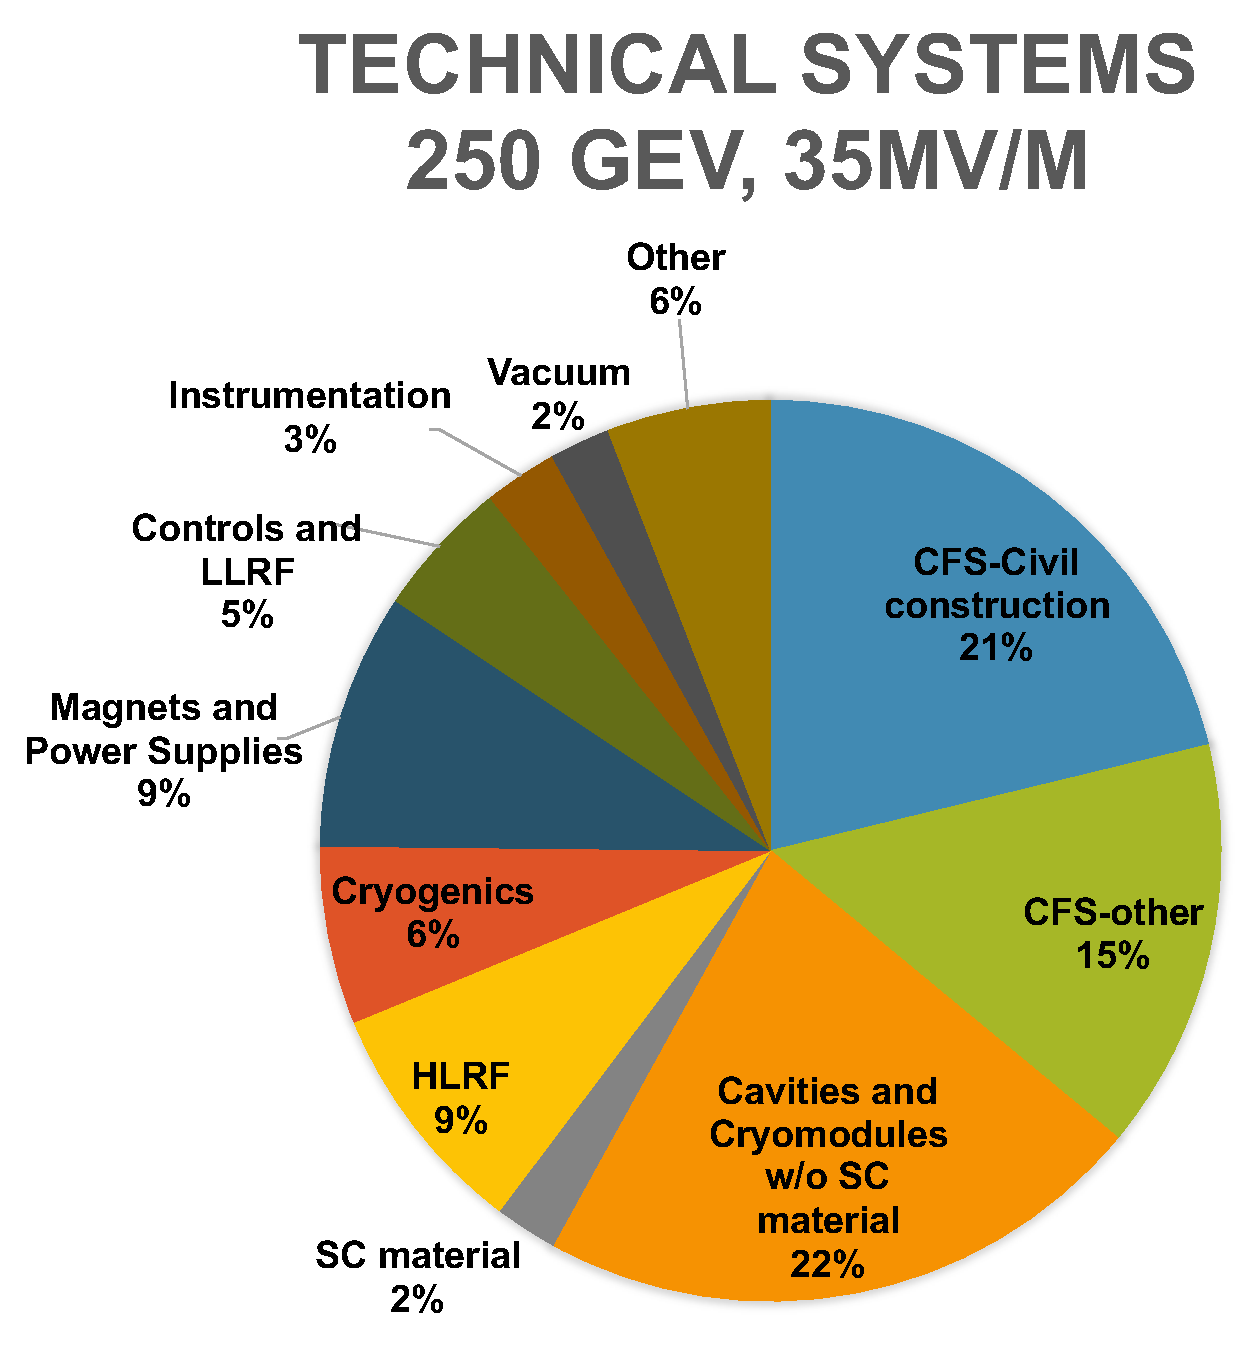
\includegraphics[width=0.4\hsize]{chapters/figures/costs-ts.pdf}
\caption{Breakdown of Value costs into accelerator systems (left) and technical systems (right) for the \siunit{250}{GeV} ILC accelerator, assuming that cost reduction measures are successful and a gradient of \siunit{35}{MV/m} can be reached.
\label{fig:costs}}
 \end{center}
 \end{figure*}


\subsection{Cost and Schedule}


%{\it 
%Description of Cost estimate and schedule - 1 page 
%
%include human resources, cost reduction effect by R\&D, operating costs
%}

For the Technical Design Report, the construction cost of the ILC accelerator was carefully evaluated from a detailed, bottom--up, WBS (Work Breakdown Structure)-based cost estimation~\cite[Sect. 15]{Adolphsen:2013kya}.
The TDR estimate distinguishes two cost categories: Value accounts for materials and supplies procured from industry and is given in ILCU (ILC Currency Unit, where $\siunit{1}{ILCU} = \siunit{1}{US\$}$ in 2012 prices), and Labour accounts for work performed in the participating institutions and is given in person--hours or person--years\footnote{One person--year corresponds to $1700$ working hours.}.

The Value of acquired goods reflects its worth in the local currency of the purchasing institution. 
Therefore, conversion of Value between currencies is performed based on Purchasing Power Parities (PPP), which are regularly evaluated and published by the OECD~\cite{OECD:2018,Eurostat:2012}, rather than currency exchange rates. 
The PPP values reflect local price levels and thus depend on the type of goods and the country, but fluctuate significantly less than currency exchange rates.
Therefore, conversions from ILCU to other currencies cannot not be made on the basis of exchange rates to the U.S. dollar, but on PPP values.

The TDR cost estimate covers the cost of the accelerator construction, assumed to last 9 years plus one year of commissioning. 
It includes the cost for the fabrication, procurement, testing, installation, and commissioning of the whole accelerator, its components, and the tunnels, buildings \etc, and the operation of a central laboratory at the site over the construction period. 
It does not, however, not cover costs during the preparation phase preceding the start of construction work (``ground breaking''), such as design work, land acquisition, infrastructure (roads, electricity, water) for the site.

Based on the TDR cost estimate, an updated cost estimate was produced for the \siunit{250}{GeV} accelerator. 
This updated cost estimate includes the cumulative effect of the changes to the design since the TDR (see Sect.~\ref{sec:design_evo}), and evaluates the cost for the reduced machine by applying appropriate scaling factors to the individual cost contributions of the TDR cost estimate.

The resulting Value estimate for the ILC accelerator at \siunit{250}{GeV} is 
\siunit{4,780-5,260}{MILCU}~\cite{Evans:2017rvt} in 2012 prices, where the lower number assumes a cavity gradient of \siunit{35}{MV/m}, while the higher number is based on the TDR number of \siunit{31.5}{MV/m}. 
In addition, \siunit{17,165}{kh} (thousand person-hours) are required of institutional Labour.

In 2018, the ILC Advisory Panel of the Japanese Ministry of Education, Culture, Sports, Science and Technoloy (MEXT) concluded its review of the ILC~\cite{ILCAP:2018}. 
For this review, costs were evaluated in Japanese Yen in 2017 prices, taking into account the local inflation for goods and construction costs.
For the purpose of this estimate, also the Labour costs were converted to Yen to yield \siunit{119.8}{G\yen}, resulting in a total range of the accelerator construction cost of \siunit{635.0 - 702.8}{G\yen}, where the range covers uncertainties in the civil construction costs (\siunit{18}{G\yen}) and of the gradient (\siunit{49.8}{G\yen}).
For the this estimate, conversion rates of $\siunit{1}{US\$} = \siunit{100}{JP\yen}$ and $\siunit{1}{\matheuro} = \siunit{1.15}{US\$}$ were assumed.

Operation costs of the accelerator and the central laboratory are estimated to be \siunit{36.6-39.2}{G\yen} (about \siunit{318-341}{M\matheuro}) per year.

% XXXXXX DISCUSS EFFECT OF COST REDUCTION R&D XXXXXX

% XXXXXX uncertainty, contingency, risk, running costs

% XXXXXX CONTINUE HERE WITH SCHEDULE   XXXXXXX












